%\documentclass[screen,citenumeric,long,10pt]{nrdoc}
\documentclass[screen,note,long,backref,indentpar]{nrdoc}
%\documentclass[twoside,citenumeric,long,10pt]{nrdoc_060418}
\usepackage{citesort}     % Virker ikke...
\usepackage{multicol}
%\usepackage{subfigure}
%\usepackage{fancyvrb}     % For crava model file
\usepackage{bm}           % For bold greek letters  --> /bm{theta}
%\usepackage{showlabels}
%\usepackage{floatflt}
%\usepackage{wrapfig}





% -------------------------------------------------
\title{CRAVA User Manual version 0.9.5}
\subject{CRAVA User Manual}
\frontpagefigure{images/FFT_flowdiagram} % No file extension.
\keywords{CRAVA, seismic, inversion, geostatistical, Bayesian, AVO, FFT}
\author{P{\aa}l Dahle\and Bj{\o}rn Fjellvoll\and Ragnar Hauge\and Odd Kolbj{\o}rnsen\and Anne Randi Syversveen\and Marit Ulvmoen }
\authorpdf{P{\aa}l Dahle, Bj{\o}rn Fjellvoll, Ragnar Hauge, Odd Kolbj{\o}rnsen, Anne Randi Syversveen and Marit Ulvmoen}
\aboutauthors{P{\aa}l Dahle is a Senior Research Scientist at NR,\\
              Bj{\o}rn Fjellvoll is a Research Scientist at NR,\\
              Ragnar Hauge  is a Chief Research Scientist at NR,\\
              Odd Kolbj{\o}rnsen is a Chief Research Scientist at NR, \\
              Anne Randi Syversveen is a Senior Research Scientist at NR and \\
              Marit Ulvmoen is a Research Scientist at NR.}
              
\availability{Open to targets}
\project{n/a}
\projectnumber{n/a}
\reportnumber{SAND/04/2009}
\target{NR, StatiolHydro, Norsar}
\researchfield{Reservoir characterisation}
% ------------------------------------------------

\makeindex

\newcommand{\vect}[1]{\ensuremath{\mathbf{#1}}}
\newcommand{\bmu}{\bm\mu}
\newcommand{\bSigma}{\mbox{\large\ensuremath{\boldsymbol{\Sigma}}}}
%\newcommand{\vp}{\ensuremath{\alpha}\xspace}     % V_{p}
%\newcommand{\vs}{\ensuremath{\beta}\xspace}      % V_{s}
\newcommand{\vp}{\ensuremath{V_p}\xspace}      % V_{p}
\newcommand{\vs}{\ensuremath{V_s}\xspace}      % V_{s}
\newcommand{\avp}{a_{\alpha}}
\newcommand{\avs}{a_{\beta}(\vec{x},t,\theta)}
\newcommand{\arho}{a_\rho(\vec{x},t,\theta)}
\newcommand{\cml}{\nu_m}
\newcommand{\cel}{\nu_e}
\newcommand{\cmt}{\nu_m}
\newcommand{\cet}{\nu_e}
%\newcommand{\cmt}{r_{\!m}}
%\newcommand{\cet}{r_{\!e}}
\newcommand{\rms}   {\textsf{Irap RMS}\xspace}
\newcommand{\crava} {\textsf{CRAVA}\xspace}
\newcommand{\storm} {\textsf{Storm}\xspace}
\newcommand{\matlab}{\textsf{MATLAB}\xspace}
\newcommand{\perl}  {\textsf{Perl}\xspace}
\newcommand{\scriptref}[2]{\ifthenelse{\boolean{screen}}
  {\hyperref[#1]{#2}}{#2 (see \ref{#1})}}

\providecommand{\autopageref}[1]{\hyperref[#1]{page~\pageref*{#1}}} %Missing definition in old version of hyperref
\def\chapterautorefname{Chapter}%
\def\sectionautorefname{Section}%
\def\subsectionautorefname{Section}%
\def\subsubsectionautorefname{Section}%
\def\paragraphautorefname{Section}%


\newcommand{\kw}[1]{\hyperref[#1]{\texttt{<#1>}}}
\newcommand{\rkw}[2]{\hyperref[#2]{\texttt{<#1>}}}
\newcommand{\rrkw}[3]{\hyperref[#3]{\texttt{<#1>}}}
%\newcommand{\rkw}[2]{\hyperref[#2]{\texttt{<#1>}}}
\newcommand{\newkw}[1]{\label{#1}\kwindex{#1}}
\newcommand{\rnewkw}[2]{\label{#2}\kwindex{#1}}
\newcommand{\rrnewkw}[3]{\label{#3}\kwindex{#1}}
\newcommand{\kwindex}[1]{\index{#1@\texttt{<#1>}}\index{element!\texttt{<#1>}}}
\newcommand{\necessary}{\small{ (necessary)}}
\newcommand{\hbracket}[1]{\texttt{<#1>}}
\newcommand{\Description}{\makebox[\rrr][l]{\textit{Description:}\xspace}}
\newcommand{\Argument}{\makebox[\rrr][l]{\textit{Argument:}\xspace}}
\newcommand{\Default}{\makebox[\rrr][l]{\textit{Default:}\xspace}}
\newlength{\rrr}
\settowidth{\rrr}{\textit{Description:}}


\newcommand{\slist}{\begin{itemize}}
\newcommand{\elist}{\end{itemize}}
    \setlength{\parindent}{0mm}
    \setlength{\parskip}{1ex}
    \renewcommand{\slist}{
    \begin{list}{}
    {
        \setlength{\itemsep}{0pt}      \setlength{\parsep}{0pt}
        \setlength{\topsep}{0pt}       \setlength{\partopsep}{0pt}
        \setlength{\itemindent}{-2em}
    }
}
\renewcommand{\elist}{\end{list}}

\newcommand{\svex}[1]{\begin{example}\label{#1}\begin{verbatim}}



\setcounter{secnumdepth}{6}
\setcounter{tocdepth}{6}
%%%%%%%%%%%%%%%%%%
\makeatletter
%%%%%%%%%%%%%%%%%%
\newcounter{subsubparagraph}[subparagraph]
\renewcommand{\thesubsubparagraph}{\thesubparagraph.\@arabic\c@subsubparagraph}
\newcommand{\subsubparagraph}{\@startsection{subsubparagraph}{6}{\parindent}
%
{3.25ex \@plus1ex \@minus .2ex}%
{-1em}%
{\normalfont\normalsize\bfseries}}
\newcommand*{\l@subsubparagraph}{\@dottedtocline{6}{14em}{7em}}
\let\subsubparagraphmark\@gobble
%%%%%%%%%%%%%%%%%%
\newcounter{subsubsubparagraph}[subsubparagraph]
\renewcommand{\thesubsubsubparagraph}{\thesubsubparagraph.\@arabic\c@subsubsubparagraph}
\newcommand{\subsubsubparagraph}{\@startsection{subsubsubparagraph}{7}{\parindent}%
{3.25ex \@plus1ex \@minus .2ex}%
{-1em}%
{\normalfont\normalsize\bfseries}}
\newcommand*{\l@subsubsubparagraph}{\@dottedtocline{7}{16em}{8em}}
\let\subsubsubparagraphmark\@gobble
\def\toclevel@subsubparagraph{6}
%%%%%%%%%%%%%%%%%%
\makeatother

%\renewcommand\floatpagefraction{.80}

\addtolength{\abovecaptionskip}{-0.4em}


\begin{document}

\maketitle

\begin{abstract}
CRAVA is a simple inversion tool, particularly suited for quick generation of first pass inversions and facies probabilities for use in geological modeling. This manual describes the theory behind, the main implementation structure, and the actual use of this program.
\end{abstract}

\tableofcontents
\clearemptydoublepage


\chapter{The \crava model}
\label{sec:theory}
\index{Bayesian inversion}

\section{Introduction}
Seismic inversion has traditionally been treated as a deterministic
problem. However, there are several uncertain aspects: There is noise
in the seismic amplitude data, and the frequency resolution is
limited, so neither high nor low frequencies can be resolved from the
seismic data alone. Using a geostatistical approach to the problem of
seismic inversion, the uncertainty may be treated in a consistent and
robust way.

The \crava program uses the Bayesian linearised AVO
inversion method of Buland {\it et. al}~\cite{geo68ab2} to take
the uncertainty in seismic data into account. The seismic data are
described using multi-normal distributions, and modelled as the seismic
response of the earth model plus an error term. The earth model and
error term are modelled as multi-normal distributions in which spatial
coupling is imposed by correlation functions. Using a Bayesian
setting, prior models for the earth and error terms are set up based
on prior knowledge obtained from well logs, and the process of seismic
inversion is reduced to that of finding a posterior distribution for
the earth given the seismic data. The linearised relationship between
the model parameters and the AVO data, makes it possible to obtain the
posterior distribution analytically.

The posterior distribution for earth model parameters \vp
(pressure-wave velocity), \vs (shear-wave velocity), and $\rho$
(density), gives a laterally consistent seismic inversion. The lateral
correlation follows the stratigraphy of the inversion interval by
following the top and base of the inversion volume. As a consequence
of the spatial coupling, the solution in each location depends on the
solutions in all other locations. From the posterior distribution the
best estimate of the model parameters and a corresponding uncertainty
can be extracted. Moreover, since the distribution is normal, kriging
can be used to match the well data, and the posterior covariance can
be computed. This spreads full frequency information in an area around
the wells. Full frequency realizations can be generated by sampling
from the posterior distribution. A set of such realizations represents
the uncertainty of the inversion.

\section{AVO}
Amplitude versus offset (AVO) inversion can be used to extract
information about the elastic subsurface parameters from the angle
dependency in the reflectivity, see e.g.,
\cite{hamp90,lort93,pan94,bula96b}. In practice, and especially for
3-D surveys, linearised AVO inversion is attractive since it can be
performed with use of moderate computer resources. Prior to a
linearised AVO inversion, the seismic data must be processed to remove
nonlinear relations between the model parameters and the seismic
response. Important steps in the processing are the removal of the
moveout, multiples, and the effects of geometrical spreading and
absorption. The seismic data should be prestack migrated, such that
dip related effects are removed. After prestack migration, it is
reasonable to assume that each single bin-gather can be regarded as
the response of a local 1-D earth model. The benefits of prestack
migration before AVO analysis are discussed in
\cite{brow92,mosh96,bula2001d}. It is further assumed that wave mode
conversions, interbed multiples and  anisotropy effects can be
neglected after processing.  Finally, the prestack gathers must be
transformed from offsets to reflection angles.

\section{Seismic model}

The seismic response of an isotropic, elastic medium is completely
described by the three material parameters $\{\vp(\vect{x},t),
\vs(\vect{x},t), \rho(\vect{x},t)\}$, where the vector $\vect{x}$
gives the lateral position (x,y), and $t$ is the vertical seismic
travel time.

The weak contrast approximation by Aki and Richards~\cite{aki80},
relates the seismic reflection coefficients $c(\vect{x},t,\theta)$
to the elastic medium, and is a linearisation of the Zoeppritz
equations (see Ref.\cite{aki80}). A continuous version of this
approximation is given by Stolt and Weglein~\cite{stolt85}:
%
\begin{equation}
\begin{split}
\label{eq:aki_c}
  c(\vect{x},t,\theta)
  & = a_{V\!p} (\theta) \frac{\partial}{\partial t}\ln\vp (\vect{x},t)\\
  & + a_{V\!s} (\vect{x},t,\theta) \frac{\partial}{\partial t}\ln\vs (\vect{x},t)\\
  & + a_\rho(\vect{x},t,\theta) \frac{\partial}{\partial t}\ln\rho(\vect{x},t),
\end{split}
\end{equation}
%
where $\theta$ is the PP reflection angle, and
%
\begin{eqnarray}
  a_{V\!p} (\theta)            &=& \frac{1}{2}\left(1 + \tan^2\theta\right), \nonumber \\
  a_{V\!s} (\vect{x},t,\theta) &=& -4 \frac{\vs^2(\vect{x},t)}
                                         {\vp^2(\vect{x},t)}\sin^2\theta, \label{a_coef_pp}\\
  a_\rho(\vect{x},t,\theta)    &=& \frac{1}{2}\left(1
                                   -4\frac{\vs^2(\vect{x},t)}{\vp^2(\vect{x},t)}
                                        \sin^2\theta\right)\nonumber
\end{eqnarray}
%
for PP reflections, and
\begin{eqnarray}
  a_{V\!p} (\theta)            &=& 0 \nonumber \\
  a_{V\!s} (\vect{x},t,\theta) &=& 2 \frac{\sin\theta}{\cos\phi}\left(\frac{\vs^2(\vect{x},t)}
                                         {\vp^2(\vect{x},t)}\sin^2\theta - \frac{\vs(\vect{x},t)}{\vp(\vect{x},t)}\cos\theta\cos\phi\right)
                                         , \label{a_coef_ps}\\
  a_\rho(\vect{x},t,\theta)    &=& \frac{\sin\theta}{\cos\phi}\left(-\frac{1}{2}+\frac{\vs^2(\vect{x},t)}
                                         {\vp^2(\vect{x},t)}\sin^2\theta + \frac{\vs(\vect{x},t)}{\vp(\vect{x},t)}\cos\theta\cos\phi\right)
                                         , \nonumber
\end{eqnarray}
for PS reflections. Here, $\phi$ is the PS reflection angle, given by$\sin\phi = \vs/\vp\sin\theta$.
These equations are linearised by replacing the ratio
$\vs(\vect{x},t)/\vp(\vect{x},t)$ with a constant value
$\bar\vp/\bar\vs$ when computing the coefficients.

The seismic data are represented by the convolutional model
%
\begin{equation} \label{timeconv}
   d_{obs}(\vect{x},t,\theta)
    =\int w(\tau,\theta) \: c(\vect{x},t-\tau,\theta) \: d\tau + e(\vect{x},t,\theta),
\end{equation}
%
where $w$ is the wavelet, and $e$ is an angle and location dependent
error term. The wavelet can be angle dependent, but independent of the
lateral position $\vect{x}$. The wavelet is assumed to be stationary
within a limited target window.

The signal-to-noise ratio is defined as the ratio of the energy in the
two terms in expression~(\ref{timeconv}), that is,
\index{signal-to-noise ratio}
%
\begin{equation} \label{SNR}
   S/N =  \| w * c\|^2 / \| e\|^2,
\end{equation}
%
\noindent
where the operator * denotes the convolution.

\section{Statistical model}
\label{sec:statmodthe}
The elastic parameters $\vp(\vect{x},t)$, $\vs(\vect{x},t)$, and
$\rho(\vect{x},t)$ are assumed to be log-normal random
fields. This means that the distribution $\vect{m}(\vect{x},t) =
\left[\ln\vp(\vect{x},t),\ln\vs(\vect{x},t),\ln\rho(\vect{x},t)\right]^T$
is multi-normal or multi-Gaussian, that is,
%
\begin{equation}
  \vect{m}(\vect{x},t) \sim
  \mathcal{N}\left(\bmu_m(\vect{x},t),\bSigma_m(\vect{x}_1,t_1;\vect{x}_2,t_2)\right),
\label{mdist}
\end{equation}
%
where $\bmu_m(\vect{x},t)$ are the expectations of
$\vect{m}(\vect{x},t)$ and $\bSigma_m(\vect{x}_1,t_1;\vect{x}_2,t_2)$
gives the covariance structure. We assume that the covariance function
is stationary and homogeneous (i.e., translationally invariant), and
can be factorised as
%
\begin{equation}
  \bSigma_m(\vect{x}_1,t_1;\vect{x}_2,t_2)
    = \bSigma_{0,m} \: \cml(\xi) \cmt(\tau), \label{sigma_m}
\end{equation}
% <
where $\cml(\xi)$ and $\cmt(\tau)$ are correlation functions
depending on the lateral and temporal distances
$\xi = \|\vect{x}_2 - \vect{x}_1\|$ and $\tau=|t_2-t_1|$,
respectively, and $\bSigma_{0,m}$ is a $3\times 3$ covariance matrix
having the variances of $\ln\vp$, $\ln\vs$ and $\ln\rho$  as diagonal
elements and their covariances off the diagonal. Any valid covariance
structures may be used.

If we let $\vect{m}$ and $\vect{d}_{obs}$ be discrete representations
of $\vect{m}(\vect{x},t)$ and $d_{obs}(\vect{x},t,\theta)$ in a time
interval, equation \eqref{timeconv} may be written in matrix
notation as
%
\begin{eqnarray}
  \vect{d}_{obs} & = & \vect{W}\vect{A}\vect{D}\vect{m} + \vect{e} \label{eq:WADm}\\
  & = & \vect{G}\vect{m} + \vect{e} \label{eq:Gm}
\end{eqnarray}
%
\noindent
where $\vect{W}$ is the matrix representation of the wavelets, $\vect{A}$ is
a matrix encompassing discrete representations of the coefficients $a_{Vp}$,
$a_{V\!s}$, and $a_\rho$, $\vect{D}$ is a differential matrix and
$\vect{G} = \vect{W}\vect{A}\vect{D}$. The
error matrix $\vect{e}$ is a time discretization of the error vector
$\vect{e}(\vect{x},t) = [e(\vect{x},t,\theta_1),\ldots,$
$e(\vect{x},t,\theta_{n_{\theta}})]^T$ and is assumed to be zero-mean
coloured Gaussian noise, that is,
%
\begin{equation}
  \vect{e}(\vect{x},t)
    \sim \mathcal{N}_{n_\theta}\left(\vect{0},
               \bSigma_e(\vect{x}_1,t_1;\vect{x}_2,t_2)\right).
\label{edist}
\end{equation}
%
The covariance of the error vector is
%
\begin{equation}
  \bSigma_e(\vect{x}_1,t_1;\vect{x}_2,t_2)
    = \bSigma_{0,e} \: \cel(\xi) \cet(\tau), \label{sigma_e}
\end{equation}
%
where $\bSigma_{0,e}$ is an $n_{\theta}\times n_{\theta}$
covariance matrix containing the noise variances for the different
reflection angles on the diagonal, and the covariances between the
angles off the diagonal. Furthermore, $\cel(\xi)$ and $\cet(\tau)$
are lateral and temporal correlation functions, similar to those
given for $\vect{m}(\vect{x},t)$ in equation~\eqref{sigma_m}.

Since the relationship between the reflection coefficients and the
elastic parameters given in equation~\eqref{eq:aki_c} is linear, and
the elastic parameters are assumed Gaussian distributed, the
reflection coefficients become Gaussian. Moreover, since the
convolution is a linear operation and we have assumed a Gaussian error
model, the seismic data given in equation~\eqref{timeconv} are also
Gaussian distributed.

For the time-discretized seismic data $\vect{d}_{obs}$, this gives us
the multi-normal distribution
%
\begin{equation}
  \vect{d}_{obs} \sim
    \mathcal{N}_{n_d}\left(\bmu_d,\bSigma_d\right),
\label{ddist}
\end{equation}
%
where
%
\begin{align}
  &\bmu_d = \vect{G}\bmu_{m},\\
  &\bSigma_d = \vect{G}\bSigma_{m}\vect{G}^T + \bSigma_e.
\end{align}
%
where all vectors and matrices are time-discretized.

This means that the simultaneous distribution for $\vect{m}$ and
$\vect{d}_{obs}$ is Gaussian, and that the distribution for $\vect{m}$
given $\vect{d}_{obs}$ can be obtained analytically using standard
theory for Gaussian distributions:
%
\begin{alignat}{2}
  &\bmu_{m|d_{obs}}    &&=\bmu_{m} +\bSigma_{m}\vect{G}^T \bSigma_{d}^{-1}
                           (\vect{d}_{obs}-\bmu_{d})     \label{eq:mupost} \\
  &\bSigma_{m|d_{obs}} &&=\bSigma_{m} - \bSigma_{m}\vect{G}^T
                           \bSigma_{d}^{-1}\vect{G}\bSigma_{m},\label{eq:sigmapost}
\end{alignat}
%
where $\bmu_{d}$ is the expected observation, that is, the
seismic response of $\bmu_m$, and $\bSigma_{d,m}$ is the
covariance matrix between logarithmic parameters and
observations. See Ref.~\cite{geo68ab1} for a detailed description on
how to compute these.

The computations given in equations~\eqref{eq:mupost}
and~\eqref{eq:sigmapost} involves the inverse of $\bSigma_{d}$. Given an
inversion volume with $n$ cells, this matrix has $n_\theta^2n^2$
elements, and for any reasonably sized volumes, inverting this matrix
is forbiddingly time consuming. However, the covariance function for a
homogeneously correlated spatial variable is diagonalised by a 3D
Fourier transform~\cite{christakos92}, and in this domain the inversion
problem can be solved independently for each frequency component. This
reduces the complexity of the computations dramatically, and the
calculation time becomes $\mathcal{O}(n\log n)$. This is illustrated
in Figure~\ref{fig:FFT-flowdiagram}. Details can be found in
Ref.~\cite{geo68ab2}
\index{FFT}
\begin{figure}[H]
  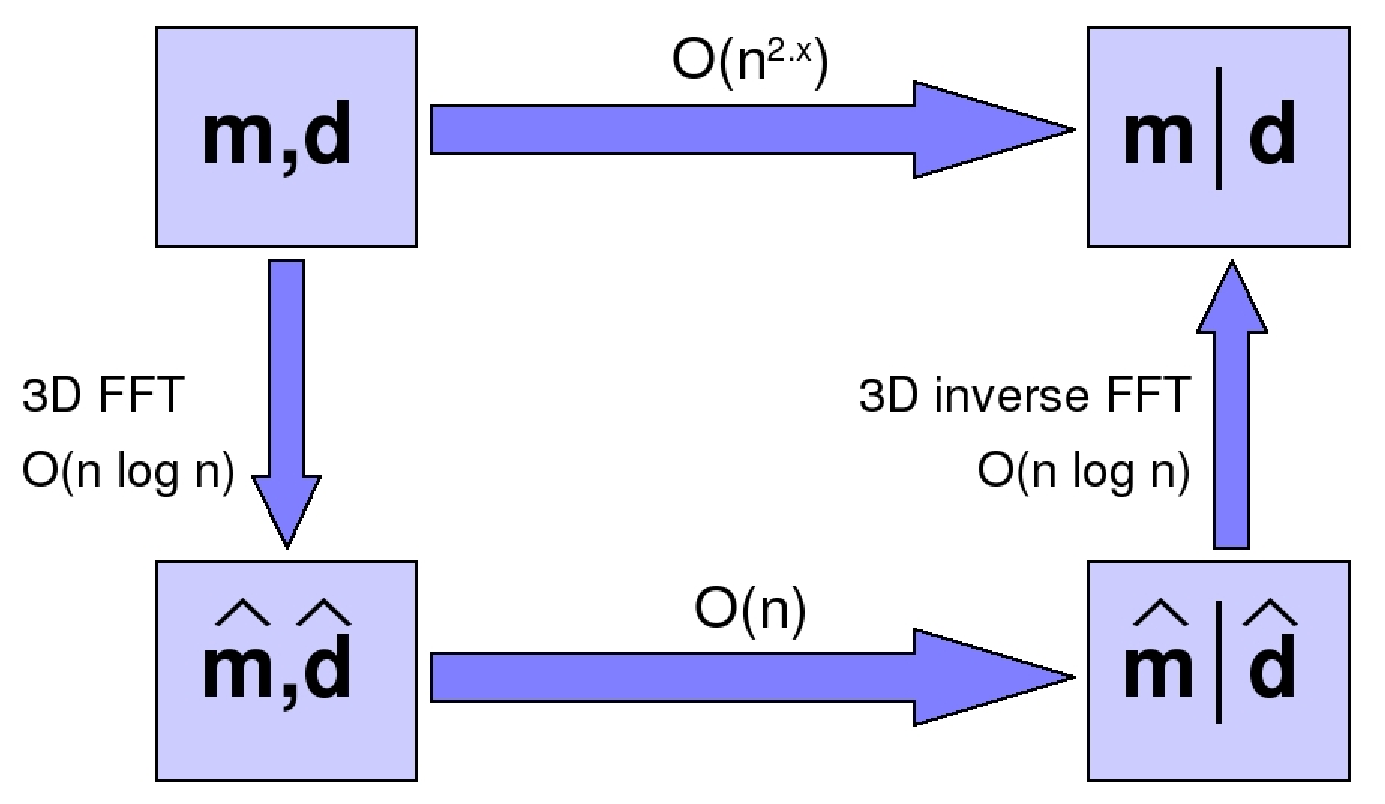
\includegraphics[width=.99\linewidth]{images/FFT_flowdiagram}
  \caption{The problem is transformed to the Fourier domain, solved
  in this domain, and back-transformed to time domain. This reduces
  the problem from a $\mathcal{O}(n^{2.x})$ to a $\mathcal{O}(n\log
  n)$ process.}
  \label{fig:FFT-flowdiagram}
\end{figure}


This seems to require that $\vect{d}$ is stationary, which would imply that the wavelet must be the same everywhere. However, we can easily divide out the wavelet from \autoref{eq:WADm} to obtain
\begin{equation}
\label{eq:ADm}
\vect{d^\prime} = \vect{A}\vect{D}\vect{m} + \vect{e^\prime},
\end{equation}
where $\vect{d^\prime}$ is the data divided by the wavelet, and $\vect{e^\prime}$ is the error divided by the wavelet. Note that we now assume that the noise after division, $e^\prime$ is stationary. Since we assume that a seismic trace only depends on the reflections in that trace, this division can be done trace by trace. This assumption relies on a rather smooth seismic response, so the lateral variations in the wavelet should be smooth. We have chosen to restrict the local wavelet changes to only allow local temporal shift and amplitude scaling.

We can also work around the stationary noise assumption, and allow $e^\prime$ to vary laterally. This is done by utilizing the nature of a Bayesian solution, which always is a tradeoff between the prior and the posterior with noisefree data. By finding the posterior for a minimal noise, we can then interpolate between this solution and the prior to find an appropriate solution for the local noise level. When doing this, we ignore correlations between the adjusted area and other values, so we require constant noise level in each trace, since the conditional correlations inside a trace are much stronger than between traces. See \autoref{sec:localnoiseimp} for details.

\subsection{Facies probabilities}
\label{sec:facprobthe}
Facies probabilities are here found by first establishing the link between facies and inversion result, $p(f_i|\bmu_{m|d,i})$, where $f_i$ is the facies at location $i$ and $\bmu_{m|d,i})$ is the inversion result at the same location. The first step is to establish the link between the well logs $\vect{m}$ and the expected seismic observations $\hat{\vect{m}}$. We get this by combining \autoref{eq:mupost} and \autoref{eq:Gm}:
\begin{eqnarray}
\bmu_{m|d_{obs}} &=&\bmu_{m} +\bSigma_{m}\vect{G}^T \bSigma_{d}^{-1}
                           (\vect{d}_{obs}-\bmu_{d}) \nonumber \\
& = & \bmu_{m} +\bSigma_{m}\vect{G}^T \bSigma_{d}^{-1}
                           (\vect{G}\vect{m}+\vect{e}-\vect{G}\bmu_m) \nonumber\\
& = & \bmu_m + \vect{A}(\vect{m}-\bmu_m)+\vect{e}^*,
\end{eqnarray}
where
\begin{eqnarray}
A & = &\bSigma_{m}\vect{G}^T \bSigma_{d}^{-1}\vect{G} \\
\vect{e}^* & \sim & \text{N}(0,\bSigma_{e^*}) \\
\bSigma_{e^*} & = & \bSigma_{m}\vect{G}^T \bSigma_{d}^{-1}\bSigma_e\bSigma_{d}^{-1}\vect{G}\bSigma_m.
\end{eqnarray}
We use this to filter the well logs and obtain the expected inversion values. For each facies, we then do a density estimation of $p(\bmu_{m|d_{obs}}|f)$ for each possible facies value $f$. This density estimation is done using a kernel smoothing approach, and by using the distribution of $\vect{e}^*$ as our kernel, we get an unbiased estimate of this distribution.

Finally we find the facies probability:
\begin{equation}
p(f=j|\bmu_{m|d_{obs}}) = \frac{p(\bmu_{m|d_{obs}}|f=j)}{\sum_i p(\bmu_{m|d_{obs}}|f=i)}.
\end{equation}.
This probability is then computed for each facies and each cell in the grid, with $\bmu_{m|d_{obs}}$ given by the inversion results. 
\newpage
\chapter{Implementation}
\label{sec:implementation}
\index{CRAVA!implementation}

Whereas the general model was explained in \autoref{sec:theory} we explain a bit more of the actual implementation details here.

\section{Using fft for inversion}
As previously stated, \autoref{eq:WADm} separates when transformed into the Fourier domain. After this transformation, the equation becomes
\begin{equation}
\label{eq:fourierinv}
\vect{\tilde{d}}(\omega,\vect{k}) = \vect{G}(\omega)\vect{\tilde{m}}(\omega,\vect{k}) + \vect{\tilde{e}}(\omega,\vect{k}))
\end{equation}
The $\tilde{ }$ denotes the 3D fourier transform, with temporal frequency $\omega$, and lateral frequency vector $\vect{k} = (k_x,k_y)$. Due to the separation, we now have a set of $n$ small equations, where $n$ is the number of grid cells in the inversion volume. Everything is still normally distributed, so the solution to this equation follows the pattern from \autoref{eq:mupost} and \autoref{eq:sigmapost}. We still must invert a data covariance matrix, but whereas this matrix had dimension $(n\cdot n_\theta)^2$ before the Fourier-transform, the matrix we must invert here is reduced to dimension $n_\theta^2$, where $n_\theta$ is the number of angle stacks. Since the time for a matrix inversion is almost cubic in size, it is much faster to invert $n$ of these small matrixes than the one large. After solving for $\vect{\tilde{m}}(\omega,\vect{k})$, we do the inverse transform of this to obtain the distribution for $\vect{m}$. The same does of course hold when we are using local wavelets that are divided out in advance, \autoref{eq:ADm}. For full details, see \cite{geo68ab2}.

\section{Local wavelet and noise}
\label{sec:nonstationaryimp}
As shown, even though the use of FFT-transform requires stationarity, we are able to work around this. Wavelets can be made local since these can be divided out before solving the problem, and locally higher noise levels can be approximated by interpolating the low-noise solution and the prior distribution.

\begin{figure}
  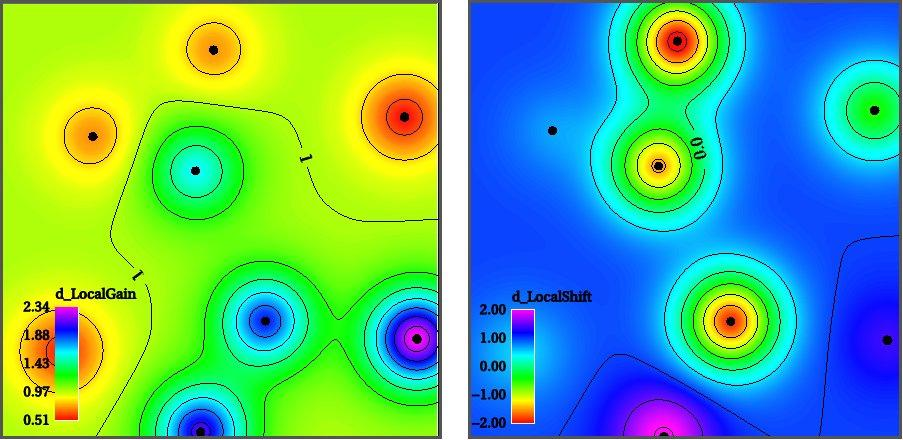
\includegraphics[width=.99\linewidth]{images/local-wavelet}
  \caption{The local gain and shift maps involved when using local wavelets}
  \label{fig:local-wavelet}
\end{figure}

\subsection{Dividing out the wavelet}
\label{sec:divwavimp}
A simple division of data by wavelet can easily be done in the Fourier domain, since the convolusion there is reduced to a multiplication, and the division can be done one frequency at a time. However, this is very unstable for frequencies where the wavelet is very weak or not present, so some stabilizing is needed.

In \crava this is done in two ways. First, we set an upper and lower cutoff frequency for the wavelet, default set to 5 and 55 Hz. Furthermore, for frequencies that fall below 10\% of the average amplitude, we set the amplitude to 10\% of average before doing the division.

\subsection{Local noise}
\label{sec:localnoiseimp}
Local noise is implemented by first finding the solution using the minimum noise level, to fulfill the stationarity requirements of the FFT algorithm. We then interpolate the values for each locations between the prior and this minimum noise posterior. When doing this interpolation, we ignore correlation between locations. This is not a problem as long as the noise varies slowly and smoothly.


For each location $\vect{x}$ the adjusted estimate $\tilde{\bmu}_{m|d_{obs}}(\vect{x})$, is found
from the inversion result $\bmu_{m|d_{obs}}(\vect{x})$ by a linear relation,
\begin{equation} \label{eq:LocalAdjustment}
\tilde{\bmu}_{m|d_{obs}}(\vect{x}) = \bmu_{m}(\vect{x}) +\vect{H_x}\left(\bmu_{m|d_{obs}}(\vect{x})-\bmu_{m}(\vect{x})\right),
\end{equation}
The matrix $\vect{H_x}$ is a shrinkage matrix, i.e. the adjusted estimate
is always closer to the prior mean than the inversion result. The matrix
$\vect{H_x}$ depends on the local error variance
 $\bSigma_{e}^x$ and error variance used in the inversion $\bSigma_{e}^0$.

To find the shrinkage matrix we first identify a matrix $\vect{G}_0$
which is such that it maps the local prior distribution to the local posterior distribution
when it is observed with the noise $\Sigma_{e}^0$, i.e.
$$ \vect{d}(\vect{x}) = \vect{G}_0\vect{m}(\vect{x})+\vect{e}_0,$$
where $\vect{e}_0\sim N\left( \vect{0},\Sigma_{e}^0\right)$.
The inversion of this expression is a linear relation
 \begin{equation} \label{eq:PSigmae}
\bmu_{m|d_{obs}} =\bmu_{m} +\vect{P}(\Sigma_{e}^0)\left(\vect{d}_{obs}-\bmu_{d}\right)
\end{equation}
where  $\vect{P}(\Sigma_{e}^0)=\bSigma_{m}\vect{G}_0^T \left( \vect{G}_0\bSigma_{m}\vect{G_0}^T+\bSigma_{e}^0\right)^{-1}$.

We then define the shrinkage matrix to be:
\begin{equation}\label{eq:H}
\vect{H_x}(\Sigma_{e}^\vect{x},\Sigma_{e}^0) = \vect{P}(\Sigma_{e}^\vect{x})\vect{P}(\Sigma_{e}^0)^{-1}.
\end{equation}
By this we mean that we remove the effect of the standard inversion and add the effect of
the locally adapted inversion. The matrix $\vect{P}(\Sigma_{e}^0)$ is not invertible,
but since the local noise always is larger than the noise in the inversion the product in
expression $\ref{eq:H}$ is always well defined.


\section{Estimation of parameters}
\label{sec:estimateimp}
The estimation routines implemented in \crava are based on straightforward and commonly used techniques. This gives fast and robust estimation, although we may run into problems if the number of data points is too small, or the data quality is too low. The quality of an estimation result is never better than the quality of the data it is based on.
\subsection{Estimating wavelet and noise}
\label{sec:waveestimp}
The wavelet estimation in \crava is based on \cite{White84}. Wavelets are estimated at well locations, where we obtain the reflection coefficients from well logs. We then use the relation
\begin{equation}
\vect{d} = \vect{w}*\vect{c}+\vect{e}
\end{equation}
where $\vect{d}$ is the seismic amplitude data, $\vect{w}$ is the wavelet, $\vect{c}$ the reflection coefficients, and $\vect{e}$ is the noise. We transform this to the Fourier domain, multiply with with the reflection coefficients, and take the expectation to get
\begin{equation}
d(\omega)\bar{c}(\omega) = w(\omega)|c(\omega)|^2
\end{equation}
Note that the convolution has disappeared, and the equation can be solved for each frequency $\omega$. However, solving this directly in the frequency domain is unstable, so we need to do a frequency smoothing. This is done by transforming $d(\omega)\bar{c}(\omega)$ and $|c(\omega)|^2$ back to time domain, multiplying with a Papoulis taper, and transforming them back to the frequency domain. This is the same as applying a local smoothing in the frequency domain. After this, we divide out $w(\omega)$, and transform back to time domain.

We find the optimal vertical shift for each well. The global wavelet is then found by taking the arithmetic average of the zero-phase wavelets, weighted by the number of samples used from each well. The noise estimate is found by generating synthetic seismic using the averaged wavelet optimally shifted in each well, and subtracting this from the seismic data. The remaining part is assumed to be noise, and we measure the noise energy from this.

When using local wavelets, we find the optimal shift and/or scale of the global wavelet at each well location. Optimal here means minimizing the noise energy. We then use kriging to interpolate this between wells, with a shift of 0 and a scale of 1 as the mean level outside the well control area.

Local noise is estimated using the local noise energies from above. We always use local shift when estimating the noise, but only use local scale if it is used in the inversion. If local scale is used, the noise is divided by this. A noise scaling factor is then computed in each well, and kriged as above.

\subsection{Estimating correlations}
\label{sec:correstimp}
We estimate correlations by first blocking the wells into the grid, and then do standard correlation estimation using
\begin{equation}
\text{Cov}(X,Y) = \text{E}(XY)-E(X)E(Y).
\end{equation}
Since we model the covariance structure as separable, we have to collapse the full time dependent covariances between parameters into one parameter covariance matrix and a temporal correlation vector. This is done simply by using the covariances at time lag 0 as our covariance matrix, and averaging the remaining time correlation vectors for the parameters.

\subsection{Estimating background model}
As with the correlation estimation, the first step is to block the wells into the modeling grid. We then filter away everything above a cutoff frequency (default 6Hz) from the well logs. The next step is to take the average of all log data in each grid layer, giving a vertical trend. This trend is then smoothed using a moving average smoother, and finally filtered with the cutoff frequency. We then use kriging of the well logs with this vertical trend as expectation to create the final background model.


\newpage
\chapter{User guide}
\label{sec:userguide}
\index{CRAVA!userguide}

In this chapter, we describe how to build a \crava model file. The model file mainly follows the XML-format, but we also use the character '\#' for commenting, meaning that the rest of the line after such a character is read as comment. XML/files are built with start- and endtags, encapsulating toher tags or values. All model files start with \texttt{<crava>}, and end with \texttt{<crava>}. An example of a model file is given in \autoref{sec:crava-model-file}.

\section{Basic inversion}
\label{sec:basicinv}
\index{inversion!basic}
A primary ability for \crava is to run simple first-pass inversions. In this section, we describe how to build a model file for a simple inversion. We focus on how to get the key information into the program, whereas more detailed controls are discussed later, in \autoref{sec:advinvusr}. The key information elements for a \crava inversion run is:
\begin{itemize}
\item \hyperref[sec:basicseis]{Seismic data}.
\item \hyperref[sec:basicwave]{Wavelet}.
\item \hyperref[sec:basicnoise]{Signal/noise ratio}.
\item \hyperref[sec:basicvol]{Inversion volume}.
\item \hyperref[sec:basicbg]{Background model}.
\item \hyperref[sec:basiccorr]{Correlation structures}.
\end{itemize}
Since \crava is designed to estimate any information that is not given, well data must also commonly be included.

\subsection{Survey information}
All information regarding the seismic data is gathered under the \kw{survey}\kwindex{survey} tag. This includes the file names for seismic data files, wavelet information and signal-to-noise ratio for each angle gather. As an example, it may look like this:
\svex{ex:survey}
<crava>
<survey>
  <segy-start-time>  2500.0 </segy-start-time>
  <angle-gather>
    <offset-angle>     16.0 </offset-angle>
    <seismic-data>
      <file-name> ../input/seismic/Cube16.segy </file-name>
    </seismic-data>
  </angle-gather>
  <angle-gather>
    <offset-angle>     28.0 </offset-angle>
    <seismic-data>
      <file-name> ../input/seismic/Cube28.segy </file-name>
    </seismic-data>
  </angle-gather>
</survey>
</crava>
\end{verbatim}
\end{example}

The seismic data can be on SegY-format, with a common offset time, given with \kw{segy-start-time}\kwindex{segy-start-time} if different from 0. The first value is used to represent the interval from start-time to start-time + time-step, so with a start-time of 100ms, and 4ms sampling, the first value is used in the grid cell covering the interval 100-104ms. Other file formats recognized by \crava is storm, Sgri and crava. 

For each available angle, the rest of the information is gathered under an \kw{angle-gather} tag, one for each offset. The actual angle is given by \kw{offset-angle}\kwindex{offset-angle}.

\subsubsection{Seismic data}
\label{sec:basicseis}
The seismic data can be given as SegY-files. By default, \crava recognizes the Seisworks, Charisma and IESX formats, but you are also allowed to define your own format using the \kw{segy-format}\kwindex{segy-format} command. For information on how to use this, see \kw{segy-format} in the reference manual chapter.

The name of the SegY file is given with \kw{file-name}, as seen in \autoref{ex:survey}. Naturally, seismic data is always required when running an inversion.

Other file formats recognized by \crava are storm, Sgri and crava. 


\subsubsection{Wavelet}
\label{sec:basicwave}
To invert the seismic data, we need a wavelet for each angle. This wavelet can be read from file, using the \kw{wavelet}\kwindex{wavelet} and \rkw{file-name}{file-name2} commands like this:
\svex{ex:wavelet}
  <angle-gather>
    <offset-angle>     16.0 </offset-angle>
    <seismic-data>
      <file-name> ../input/seismic/Cube16.segy </file-name>
    </seismic-data>
    <wavelet>
      <file-name> ../input/wavelets/wavelet16.txt </file-name>
    </wavelet>
  </angle-gather>
\end{verbatim}
\end{example}

We can read wavelets on Swav and asc format.

If the \kw{wavelet} command is not given, or given without \kw{file-name}, the wavelet is estimated. See \autoref{sec:waveestimp} for how this is done. If the wavelet is given on file, but unscaled, the command \kw{scale}\kwindex{scale} should be used if the scale is known, otherwise, the scale can be estimated by using the \kw{estimate-scale}\kwindex{estimate-scale} command. If none of these are specified, the wavelet will be used as it is on file.

\subsubsection{Signal/noise ratio}
\label{sec:basicnoise}
This ratio is given with \kw{signal-to-noise-ratio}\kwindex{signal-to-noise-ratio}. If this command is not given, the ratio is estimated. Note that we define the signal to noise ratio as the data variance divided by the error variance, where the data variance is model variance plus error variance.

\subsection{Inversion volume}
\label{sec:basicvol}
The volume used for inversion is given horizontally by a rectangle, and vertically bounded by a top and base surface. It is defined by the command \kw{output-volume}\kwindex{output-volume} under \kw{project-settings}. Typically, it may look something like this:
\svex{ex:volume}
<crava>
<project-settings>
  <output-volume>
    <utm-coordinates>
      <reference-point-x>  403050.0   </reference-point-x>
      <reference-point-y> 7211900.0   </reference-point-y>
      <length-x>              500.0   </length-x>
      <length-y>              500.0   </length-y>
      <angle>                  23.627 </angle>
      <sample-density-x>       50.0   </sample-density-x>
      <sample-density-y>       50.0   </sample-density-y>
    </utm-coordinates>

    <interval-two-surfaces>
      <top-surface>
        <time-file>     ../input/horizons/FlatTop_3100ms.storm </time-file>
      </top-surface>
      <base-surface>
        <time-file>    ../input/horizons/FlatBase_3600ms.storm </time-file>
      </base-surface>
      <number-of-layers> 125 </number-of-layers>
    </interval-two-surfaces>
  </output-volume>
</project-settings>
</crava>
\end{verbatim}
\end{example}

\subsubsection{Lateral extent}
The lateral extent of the inversion volume is given under one of the
the commands \kw{area-from-surface}\kwindex{area-from-surface},
\kw{utm-coordinates}\kwindex{utm-coordinates}, or
\kw{inline-crossline-numbers}\kwindex{inline-crossline-numbers}. The
command \kw{utm-coordinates} describes a rectangle, which may be
rotated relative to the seismic data. It has the following parameters,
which must all be specified: 
\begin{itemize}
\item \kw{reference-point-x}\kwindex{reference-point-x} is the UTM x-coordinate of one corner of the area.
\item \kw{reference-point-y}\kwindex{reference-point-y} is the UTM y-coordinate of the same corner.
\item \kw{length-x}\kwindex{length-x} is the extent of the area along the local x-axis.
\item \kw{length-y}\kwindex{length-y} is the extent of the area along the local y-axis.
\item \kw{angle}\kwindex{angle} is the angle between the direction of the UTM x-axis and the local x-axis. Positive angles are counterclockwise.
\item \kw{sample-density-x}\kwindex{sample-density-x} is the length of one grid cell along the local x-axis.
\item \kw{sample-density-y}\kwindex{sample-density-y} is the length of one grid cell along the local y-axis.
\end{itemize}
Note that if the grid has the same rotation as the input SegY cubes with seismic data, output SegY cubes will have correct inlines and crosslines. Otherwise, these numbers are just counting from the initial corner.
The command \kw{area-from-surface} contains only one parameter, \kw{file-name}\kwindex{file-name}, the name of a storm surface file defining the lateral extent of the inversion volume.
The last way to define the inversion area is by the command \kw{inline-crossline-numbers}\kwindex{inline-crossline-numbers}. By this command, the following parameters can be used:
\begin{itemize}
\item \kw{il-start}\kwindex{il-start} is the starting inline number.
\item \kw{il-end}\kwindex{il-end} is the ending inline number.
\item \kw{xl-start}\kwindex{xl-start} is the starting crossline number.
\item \kw{xl-end}\kwindex{xl-end} is the ending crossline number.
\item \kw{il-step}\kwindex{il-step} is the inline interval.
\item \kw{xl-step}\kwindex{xl-step} is the crossline interval.
\end{itemize}
The parameters \kw{il-start} and \kw{xl-start} must be set if this command is used, the other parameters are optional. If they are not given, the numbers are taken from the Segy file containing the first seismic cube.

The area commands may be skipped altogether. The area will then be taken from the first input seismic data file, and defined as the smallest rectangle that covers all present traces.

\subsubsection{Top and bottom surfaces}
The vertical extent is normally given by a top and a base surface in time, under the command \kw{interval-two-surfaces}\kwindex{interval-two-surfaces}, as shown in \autoref{ex:volume}. The file name for the top surface is given under command \kw{top-surface}\kwindex{top-surface}, \kw{time-file}, and the base surface is given similarly under \kw{base-surface}\kwindex{base-surface}, \kw{time-file}. The file format is binary storm or ASCII irap.

These surfaces also define the default lateral correlation direction for the elastic parameters, with the correlation being parallel to the top surface at the top, and base surface at the base. Between this, we create a top- and base-conform grid, so that the number of grid cells in each trace is constant, although the interval thickness may vary. This is shown in \autoref{fig:conformgrid}. The inversion may be unstable if the resolution varies too much in different traces, so we recommend that no trace interval is larger than twice the shortest interval.
\begin{figure}[H]
  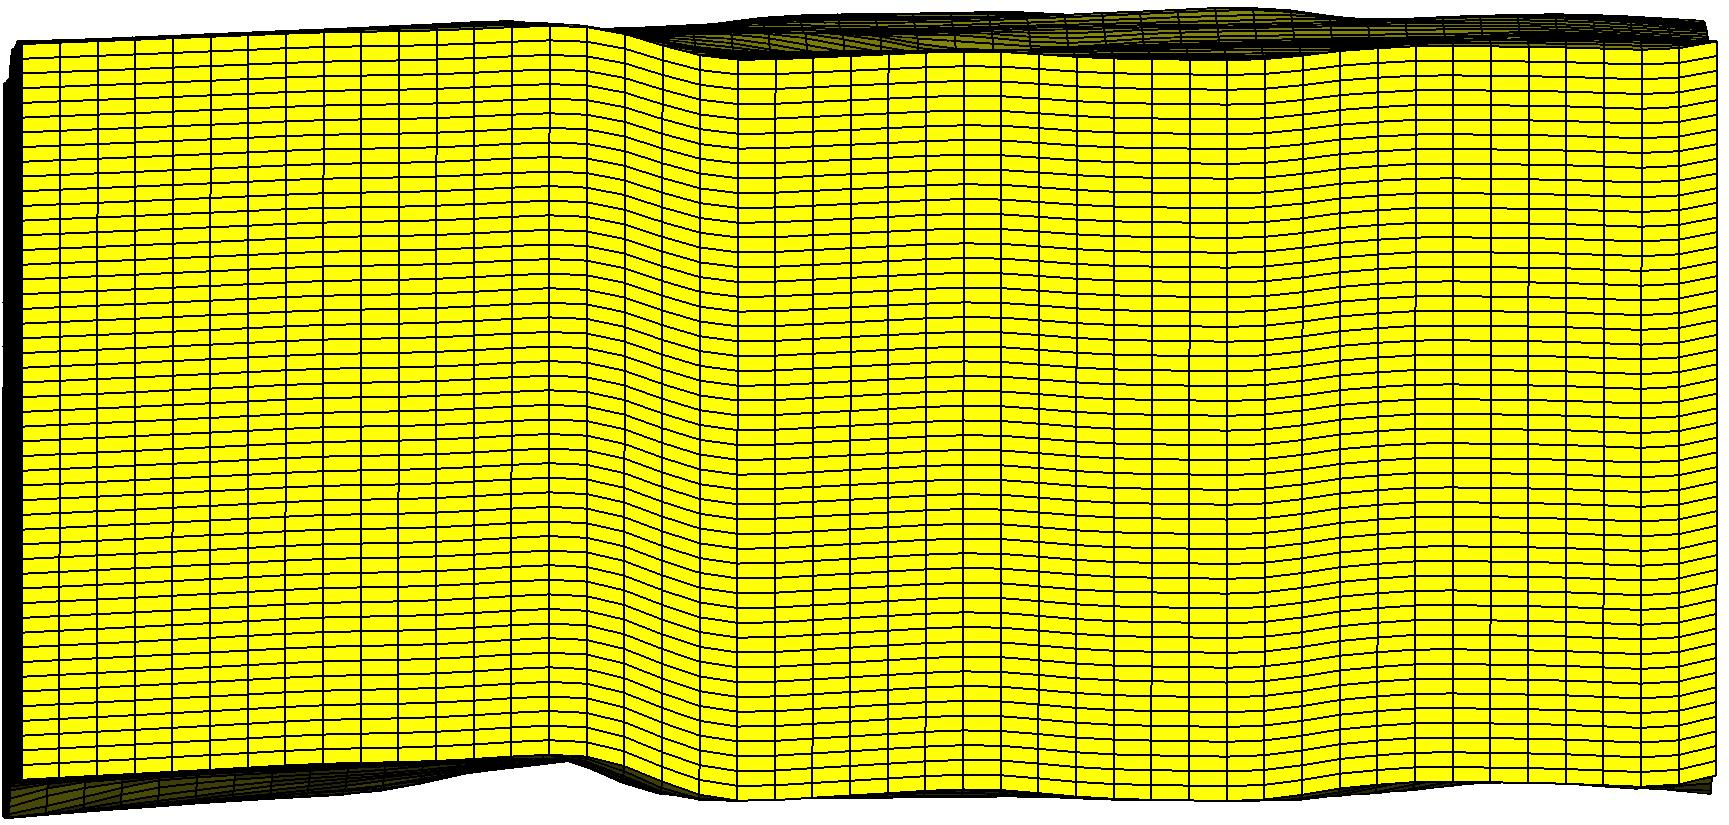
\includegraphics[width=.99\linewidth]{images/conformgrid}
  \caption{The layer structure of a top- and base-conform grid.}
  \label{fig:conformgrid}
\end{figure}
\begin{figure}
  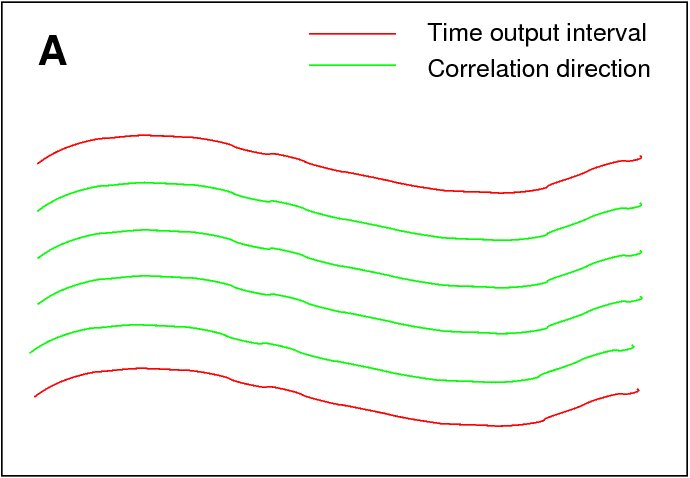
\includegraphics[width=.49\linewidth]{images/A_correlation_parallel}
  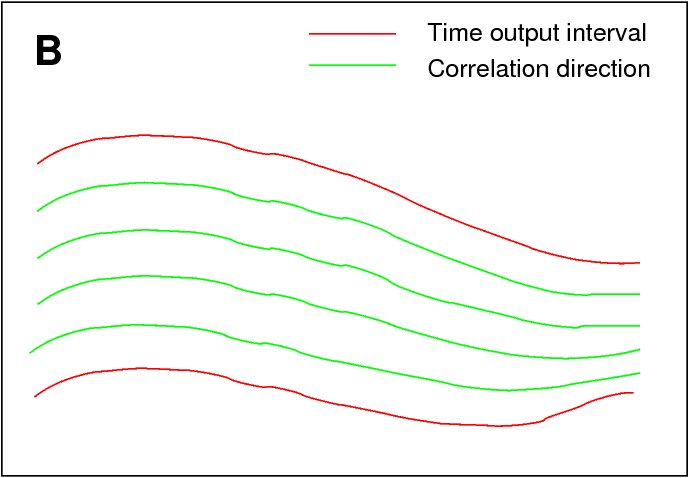
\includegraphics[width=.49\linewidth]{images/B_correlation_proportional}\\
  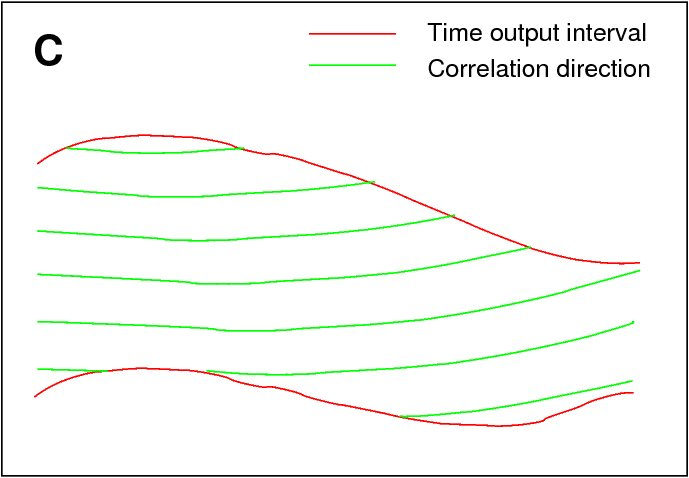
\includegraphics[width=.49\linewidth]{images/C_correlation_parallel_timecut}
  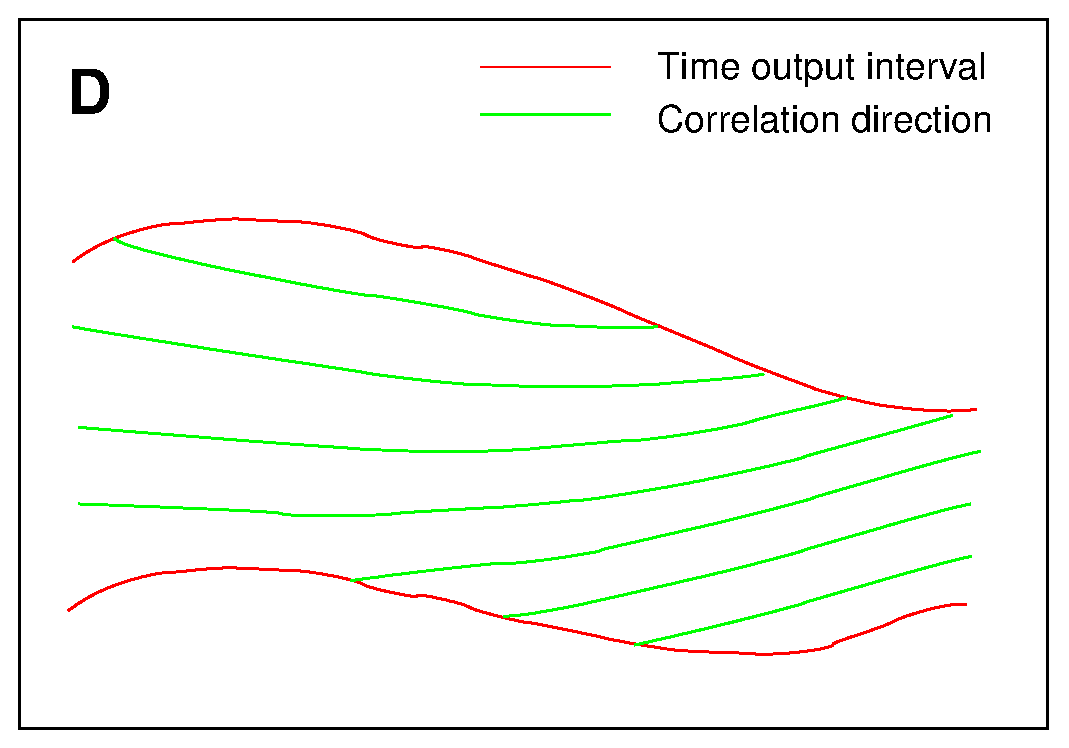
\includegraphics[width=.49\linewidth]{images/D_correlation_proportional_timecut}
  \caption{The layer structure of a (A) parallel top and base,
    (B) top- and base-conform compaction grid (C) Uniform correlation structure in a cut grid (D) Compactional correlation structure in a cut grid.}
  \label{fig:inversion-interval-types}
\end{figure}
By specifying a correlation surface, the correlation direction can be independent of the interval surfaces, see \autoref{sec:basiccorr}. If this is done, there are no restrictions on the differences in interval thickness.

If only one surface is known, the command \kw{interval-one-surface} can be used to invert an interval with top and base parallel to this surface. See \autoref{interval-one-surface} in the reference guide for more details. Note that depth conversion and correlation surfaces will not be available in this mode, so the lateral correlation will be parallel to this surface.

\subsubsection{Depth conversion}\label{sec:depthconvusr}
The \kw{output-volume} command is also where the depth conversion is specified, since this also constitutes a volume although in depth. Since the lateral area obviously is the same, the additional information for depth conversion is given under \kw{interval-two-surfaces}. To do the depth conversion, one of the following must be given:
\begin{itemize}
\item Reference surface in depth (either top or base), and a velocity cube.
\item Both top and base surface in depth. In this case, we assume constant velocity along each trace, computed from the time and depth surfaces.
\item Both top and base surface in depth, and a velocity cube. In this case, we use the cube for relative velocity in a trace, and scale it to match the interval length.
\end{itemize}

Reference surfaces in depth are given with \kw{depth-file}\kwindex{depth-file} under \kw{top-surface} and/or \kw{base-surface}. The velocity cube can be read from a storm-file with the command \kw{velocity-field}\kwindex{velocity-field}. Alternatively, the command \kw{velocity-field-from-inversion}\kwindex{velocity-field-from-inversion} can be used to specify that Vp from inversion should be used for velocity. With depth conversion, the \kw{interval-two-surfaces} command may look like this:
\svex{ex:depthconv}
    <interval-two-surfaces>
      <top-surface>
        <time-file>     ../input/horizons/FlatTop_3100ms.storm </time-file>
        <depth-file>    ../input/horizons/FlatTop_3100ms.storm </depth-file>
      </top-surface>
      <base-surface>
        <time-file>    ../input/horizons/FlatBase_3600ms.storm </time-file>
        <depth-file>   ../input/horizons/FlatBase_3800ms.storm </depth-file>
      </base-surface>
      <velocity-field>        ../input/velocity/velocity.storm </velocity-field>
      <number-of-layers>                                   125 </number-of-layers>
    </interval-two-surfaces>
\end{verbatim}
\end{example}

\subsection{Prior model}
Since seismic data only contain information about relative elastic parameters, the absolute level needs to be set with a background model. In a Bayesian inversion setting, the background model is the prior expectation. We also need the prior covariance, which is given by the covariance of the parameters, the lateral correlation and the temporal correlation, as described in \autoref{sec:statmodthe}. In the model file, all this is gathered under the \kw{prior-model}\kwindex{prior-model} command, which may look something like this:
\svex{ex:priormodel}
<crava>
<prior-model>
  <background>
    <vp-file>
      ../../input/background/CravaBgVp.storm
    </vp-file>
    <vs-file>
      ../../input/background/CravaBgVs.storm
    </vs-file>
    <density-file>
      ../../input/background/CravaBgRho.storm
    </density-file>
  </background>
  <lateral-correlation>
    <variogram-type> genexp </variogram-type>
    <power>       1 </power>
    <angle>       0 </angle>
    <range>    2500 </range>
    <subrange> 2500 </subrange>
  </lateral-correlation>
</prior-model>
</crava>
\end{verbatim}
\end{example}

\subsubsection{Background model}
\label{sec:basicbg}
The background model is given under the \kw{background}\kwindex{background} command. It can be given from file, using \kw{vp-file}\kwindex{vp-file}, \kw{vs-file}\kwindex{vs-file} and \kw{density-file}\kwindex{density-file}. These files should either be on Storm, crava, Sgri or SegY format. Alternatively, constant values can be used for background model, specified with \kw{vp-constant}\kwindex{vp-constant}, \kw{vs-constant}\kwindex{vs-constant} and \kw{density-constant}\kwindex{density-constant}. Any combinations of files and constants are also ok. If none of these are given, the background model will be estimated.
\subsubsection{Covariances}
\label{sec:basiccorr}
As shown in \autoref{sec:statmodthe} the prior covariance structure for the elastic parameters consists of three parts:
\begin{enumerate}
\item A 3x3 covariance matrix for pointwise covariance between the parameters. May be read from ascii file using the command \kw{parameter-correlation}\kwindex{parameter-correlation}.
\item A temporal correlation vector, length equal to number of layers in grid, $n_t$. May be read from ascii file using the command \kw{temporal-correlation}\kwindex{temporal-correlation}.
\item A lateral correlation structure. May be given as a variogram using the command \kw{lateral-correlation}.
\end{enumerate}
By default, the two first are estimated from well data, and the lateral correlation structure is set to a isotrope exponential variogram with range 1000. The reason for the latter choice is that this is hard to estimate, see \autoref{sec:correstimp} for details. The most common to override is the lateral correlation, where the variogram used for petrophysical modelling is a good choice.
\subsection{Well data}
Unless all information about wavelet, signal to noise and correlations are specified, well data are needed for estimation. Wells are given with the command \kw{well-data}\kwindex{well-data}, and may look like this:
\svex{ex:welldata}
<crava>
<well-data>
  <log-names>
    <time>    TWT  </time>
    <dt>      DT   </dt>
    <dts>     DTS  </dts>
    <density> RHOB </density>
  </log-names>
  <well>
    <file-name> ../input/logs/ed6406_3-3_cut.rms    </file-name>
  </well>
  <well>
    <file-name> ../input/logs/ed6506_12-3_cut.rms   </file-name>
  </well>
  <well>
    <file-name> ../input/logs/ed6506_12-8_cut.rms   </file-name>
  </well>
  <well>
    <file-name> ../input/logs/ed6506_12-S4H_cut.rms </file-name>
  </well>
</well-data>
</crava>
\end{verbatim}
\end{example}
There are two main elements here. The first is a well log
interpretation, given by \kw{log-names}, which tells \crava which
headers to look for. The following logs are needed: 
\begin{itemize}
\item Two way time log, specified with \kw{time}\kwindex{time}.
\item Vp log, either given by \kw{vp}\kwindex{vp} or \kw{dt}\kwindex{dt}. The latter is used for DT-logs.
\item Vs log, either given by \kw{vs}\kwindex{vs} or \kw{dts}\kwindex{dts}. The latter is used for DTS-logs.
\item Density log, given by \kw{density}\kwindex{density}.
\end{itemize}
In addition, if facies probabilities are computed, a facies log is
needed. This is specified with \kw{facies}\kwindex{facies}. 

The wells are given with the command \kw{file-name} under
\kw{well}\kwindex{well}, which is given once for each well. The reason
for this is that additional information may be given for each
well. Well files should be on RMS-format. 

Each well may be moved to its optimal location using \kw{optimize-location-to}\kwindex{optimize-location-to} under \kw{well}\kwindex{well}, taking the arguments \rkw{angle}{angle3}\kwindex{angle} and \kw{weight}\kwindex{weight} allowing the user to assign different weights to the different angle gathers for each well. The maximum allowed offset and vertical shift for moving wells is specified in \kw{maximum-offset}\kwindex{maximum-offset} and \kw{maximum-shift}\kwindex{maximum-shift} under \kw{well-data}, with default values of 250 m and 11 ms, respectively.

\subsection{Output}
Output is controlled under \kw{io-settings}\kwindex{io-settings} under
\kw{project-settings}. Here, you may set the output directory using
\kw{output-directory}\kwindex{output-directory}, and a prefix for all
output files using
\kw{file-output-prefix}\kwindex{file-output-prefix}. This prefix will
be added to all output files. 

Except for the log file which is placed directly under the
output directory, all files output by crava are placed in
sub-directories. These sub-directories are 

\svex{ex:output-directoies}
output-directory / wells 
                 / background 
                 / wavelets 
                 / seismic 
                 / velocity 
                 / correlations 
                 / inversionresults 
\end{verbatim}
\end{example}

There are two main output formats: Grid output, controlled by
\kw{grid-output}\kwindex{grid-output}, and well output controlled by
\kw{well-output}\kwindex{well-output}. The output section may look
something like this: 
\svex{ex:iosettings}
<crava>
<project-settings>
  <io-settings>
    <file-output-prefix> CRAVA_ </file-output-prefix>
      <grid-output>
        <format>
          <segy> yes </segy>
        </format>
        <domain>
          <time>  yes </time>
          <depth> yes </depth>
        </domain>
        <elastic-parameters>
          <vp> yes </vp>
          <vs> yes </vs>
          <density> yes </density>
          <background> yes </background>
        </elastic-parameters>
      </grid-output>
      <well-output>
        <wells> yes </wells>
        <blocked-wells> yes </blocked-wells>
      </well-output>
  </io-settings>
</project-settings>
</crava>
\end{verbatim}
\end{example}

\subsubsection{Grid output}\kwindex{grid-output}
Different elastic parameters can be given as grid output. In addition, estimated background model may be written as grids. This is controlled by the \kw{elastic-parameters}\kwindex{elastic-parameters} command under \kw{grid-output}. See \autoref{elastic-parameters} for a full list of possible grids. If this command is not used, Vp, Vs and density will be written. Output of original and synthetic seismic data can be given by the \kw{seismic-data}\kwindex{seismic-data} command. Other output grids are given by the command \kw{other-parameters}{kwindex{other-parameters}, for example correlations.

The grid format may be controlled using \kw{format}\kwindex{format}. Here the yes/no parameters \kw{storm}, \kw{segy}, \kw{sgri}, \kw{crava} and \kw{ascii} can be used to decide if grids should be written on storm- (RMS), segy-, Sgri-, crava- or ascii-format. You may choose several formats for one run; all grids will be written on all selected formats. Note that correlation grids make sense only in storm format. Default output format is storm. The crava format is a binary format only to be used with Crava. It can be read and written from \crava, and is useful if the output from a \crava run should be used as input to another \crava run because the format is fast to read.

By using the \kw{domain}\kwindex{domain} option, output may be written in time domain (\kw{time}) or depth domain (\kw{depth}, requires parameters set under \kw{output-volume}, see \autoref{sec:depthconvusr}), or both. Again, correlation grids only make sense in time domain, which is default.

\subsubsection{Well output}\kwindex{well-output}
Some versions of filtered elastic parameters (Vp, Vs and density) in wells can be generated by the \kw{well-output} command. The logs written are
\begin{itemize}
\item Raw elastic logs.
\item Elastic logs filtered to background frequency.
\item Elastic logs filtered to seismic frequency.
\item Elastic logs filtered with facies prediction filter (if available).
\item Facies log (if available).
\end{itemize}
The wells can either be written with original sampling density, using \kw{wells}, or matching the internal grid resolution, using \kw{blocked-wells}.

\subsection{Actions}
The final information that is needed for a \crava run is what the run is supposed to do. This is controlled by \kw{actions}\kwindex{actions}. The \kw{mode} keyword defines the purpose of this run. and should be set to "inversion" when doing inversion. Other options are "estimation", see \autoref{sec:estimateusr} and "forward", see \autoref{sec:forwardusr}. When inversion is chosen, \kw{inversion-settings}\kwindex{inversion-settings} can be used to control basic aspects of the inversion. It may look something like this:
\svex{ex:action}
<crava>
<actions>
  <mode> inversion </mode>
  <inversion-settings>
    <prediction> yes </prediction>
    <simulation>
      <seed> 210471 </seed>
      <number-of-simulations> 10 </number-of-simulations>
    </simulation>
  </inversion-settings>
</actions>
</crava>
\end{verbatim}
\end{example}

The command \kw{prediction}\kwindex{prediction} can be used to turn predictions on or off. By default, the prediction will be generated. A number of full frequency stochastic realisations of the inversion by specifying \kw{number-of-simulations}\kwindex{number-of-simulations} under \kw{simulation}\kwindex{simulation}. The seed for the random generator can also be given here, with the \kw{seed}\kwindex{seed} command. Changing the seed will give a new set of realisations.
\section{Advanced inversion options}
\label{sec:advinvusr}
Although \crava is mainly intended as a simple and fast inversion tool, there are still some options to control the inversion, and using more sophisticated approaches. Most of these are covered here, see also \autoref{advanced-settings} for details about \kw{advanced-settings}.
\subsection{Non-stationary wavelet and noise}
Although the FFT-algorithm which is at the core of \crava requires
stationarity, this does not mean that the entire inversion has to be
stationary, as discussed in \autoref{sec:nonstationaryimp}. We allow
lateral variations in wavelet amplitude, wavelet shift and signal to
noise ratio. 

Unlike the basic level, where parameters that were not specified
automatically got estimated, use of local wavelets or noise must be
explicitly triggered. For wavelets, this is done with the
\kw{local-wavelet}\kwindex{local-wavelet} command under
\kw{wavelet}. There are four possible commands under
\kw{local-wavelet}: 
\begin{enumerate}
\item \kw{shift-file} gives a file name for a map giving the local shifts. The file must be on storm format.
\item \kw{estimate-shift} will estimate a local shift map when set to "yes".
\item \kw{scale-file} gives a file name for a map giving the local scale. The file must be on storm format.
\item \kw{estimate-scale} will estimate a local scale map when set to "yes".
\end{enumerate}
Naturally, the shift can not be both given and estimated, the same
holds for scale. Note that you may choose to use only shifts, omitting
both scale keywords, or use only scale. 

The local noise is triggered similarly, by using one of these two
commands under \kw{angle-gather}: 
\begin{enumerate}
\item \kw{local-noise-scaled} gives a file with the local scaling of
  the signal to noise ratio, on storm format. 
\item \kw{estimate-local-noise} estimates the local scaling of the
  signal to noise ratio if set to "yes". 
\end{enumerate}

\subsection{PS-seismic and reflection approximations}
By default, \crava assumes that the input seismic data are PP, but PS
data can also be used. For both cases, we use  linearized
Aki-Richards, see \autoref{eq:aki_c}. The type of seismic data is
indicated by using the \kw{type}\kwindex{type} command
under\kw{seismic-data}. Here, \kw{type} should be either "pp" or
"ps". Note that PS data must also be aligned in PP-travel time, as no
such alignment is done internally by \crava. 

Instead of using the default reflection approximation, the user may
supply the parameters to compute the reflections. We always assume
that for a given angle and seismic type, the reflections can be
computed from the equation 
\begin{equation}
\begin{split}
  c(\vect{x},t,\theta)
  & = a_{V\!p} (\theta) \frac{\partial}{\partial t}\ln\vp (\vect{x},t)\\
  & + a_{V\!s} (\vect{x},t,\theta) \frac{\partial}{\partial t}\ln\vs (\vect{x},t)\\
  & + a_\rho(\vect{x},t,\theta) \frac{\partial}{\partial t}\ln\rho(\vect{x},t).
\label{eq:linrefl}
\end{split}
\end{equation}
The coefficients $a_{V\!p}$, $a_{V\!s}$ and $a_\rho$ can be read from
file, using the \kw{reflection-matrix}\kwindex{reflection-matrix}
command under \kw{advanced-settings}. This file should have one line
for each seismic data file, and each line should have the three
coefficients for one set of seismic input data. The order of the lines
should be the same as the order of the seismic data in the \kw{survey}
command. 

\subsection{Well quality checks}
Well logs are often faulty, and \crava has some safety mechanisms to
detect this. The primary mechanism is to detect extreme values, and
set these missing. The default upper and lower bounds are shown in
\autoref{tab:logminmax}. These can be overridden using the command
\kw{allowed-parameter-values}\kwindex{allowed-parameter-values} under
\kw{well-data}. Here, \kw{minimum-vp}, \kw{minimum-vs},
\kw{minimum-density} and the corresponding maximum values can be
given. 
\begin{table}
\begin{tabular}{|lrr|}
\hline
& Min & Max \\
\hline
Vp & 1300 & 7000 \\
Vs &  200 & 4200 \\
Density & 1.4 & 3.3
\end{tabular}
\caption{Default intervals for valid log values.\label{tab:logminmax}}
\end{table}


Some logs may stay within reasonable values, but have too much or too
little variation, also indicating that something is wrong. For each
log, the variance of the logarithm of the log minus the background is
computed, and if it is outside reasonable bounds, this triggers an
error. The default bounds are shown in
\autoref{tab:logvarminmax}. These can also be overridden with
\kw{allowed-parameter-values}, using \kw{minimum-variance-vp} and so
on. 
\begin{table}
\begin{tabular}{|lrr|}
\hline
& Min & Max \\
\hline
Var(ln(Vp)) & $5*10^{-4}$ & $250*10^{-4}$ \\
Var(ln(Vs)) & $10*10^{-4}$ & $500*10^{-4}$ \\
Var(ln(Density)) & $2*10^{-4}$ & $100*10^{-4}$ \\
\end{tabular}
\caption{Default intervals for valid log variances.\label{tab:logvarminmax}}
\end{table}

\subsection{Generate synthetic seismic from inversion data}
It is possible to generate synthetic seismic by a forward modeling
with the Vp, Vs and density resulting from the inversion. This is done
by the command  \kw{synthetic} under \kw{seismic-data} under
\kw{grid-output}, \kw{io-settings},  in command
\kw{project-settings}. 

\section{Estimation}
\label{sec:estimateusr}
As mentioned, \crava can estimate many of the needed parameters. There
are several commands that control the estimation behavior for
wavelets, noise and background model. Note that the correlations will
always be estimated as explained in \autoref{sec:estimateimp} from all
available well logs, and do not have any further controls. 

\subsection{Estimation mode}
If you only want to do the estimation, in order to check the quality
of the estimates, you can use "estimate" in the \kw{mode}
command. Using this, \crava will perform the initial model building
tasks and estimate needed information, but terminate once all
information needed for inversion is estimated. When running in
estimation mode, you can also control the main estimation aspects
using the \kw{estimation-settings}\kwindex{estimation-settings}
command. This allows you to control which of the main estimation tasks
should be carried out, setting yes or no for
\kw{estimate-correlations}, \kw{estimate-wavelet-or-noise} or
\kw{estimate-background}. Parameters with a "no" will not be estimated
unless needed for other estimations. Note that in estimation mode, all
estimated parameters are written to file, regardless of output
settings. 
\subsection{Wavelet and noise estimation}
Wavelets and noise are estimated together. These parameters will only
be estimated from wells that are vertical or close to vertical, since
this allows comparing synthetic seismic from well logs with one or a
couple of traces, and thus reduces alignment issues. The angle limit
can be controlled by the
\kw{maximum-deviation-angle}\kwindex{maximum-deviation-angle} command
under \kw{well-data}. In addition, wells can be excluded individually,
by setting \kw{use-for-wavelet-estimation} to "no" under \kw{well}. 

By default, the wavelet and noise are estimated in the region between
the top and bottom surface for the inversion area. This may be further
limited using the \kw{wavelet-estimation-interval} command under
\kw{survey}, where a separate set of restricting surfaces are given
with \kw{top-surface-file} and \kw{base-surface-file}. Since these are
under \kw{wavelet}, they can be different for each angle. 

Some wavelet estimation options are also found under \kw{advanced-settings} under \kw{project-settings}. These are
\begin{itemize}
\item \kw{wavelet-tapering-length} which controls the length of the wavelet (in ms).
\item \kw{minimum-relative-wavelet-amplitude} which finds the wavelet
  length, by setting the cutoff size for edge peaks relative to center
  peak. 
\item \kw{maximum-wavelet-shift} which controls how far the wavelet
  can be shifted locally, see \autoref{sec:waveestimp}. 
\end{itemize}

\subsection{Background model estimation}
The background model is estimated as a low frequency vertical
trend. The trend is given in relative depth in the inversion volume,
so the trend value along the top and bottom surface is constant. At
well locations, the trend is kriged to the well logs. By default, all
wells are used background model estimation, but can be excluded by
using \kw{use-for-background-trend} under \kw{well} for individual
wells. 

The background estimation can be controlled by some commands under
\kw{background}\kwindex{background}. These are: 
\begin{itemize}
\item \kw{velocity-field} takes an external velocity field, typically
  from migration, and uses as Vp background, kriged to low frequency
  Vp well logs. 
\item \kw{lateral-correlation} gives a variogram for the
  kriging. Larger ranges extends well data further away from wells. 
\item \kw{high-cut} allows specification of a maximum frequency for
  the background model. 
\end{itemize}

\section{Facies prediction}
An important feature in \crava is the ability to create facies
probabilities. This requires that \kw{mode} is set to "inversion", and
is triggered by the \kw{facies-probabilities} command under
\kw{inversion-settings}. The value given here should be either
"absolute" or "relative", corresponding to probability computations
based on absolute or relative inverted parameters. If the distribution
for elastic parameters for each facies is constant over the inversion
volume, using absolute values is more stable. However, if there are
trends in the elastic parameters, the relative values are more
robust. 

The facies probabilities are computed based on the inversion results
and a distribution for inversion values given facies computed from
filtered well logs, where the filter is defined by the inversion. See
\autoref{sec:facprobthe}. Probability cubes will be computed for all
facies seen in wells, and an additional undefined probability cube is
also generated, indicating areas where the inversion values are too
far away from well data to make reliable predictions. 

Except from the trigger in \kw{inversion-settings}, all parameters
related to facies probabilities are given under
\kw{facies-probabilities}\kwindex{facies-probabilities} under
\kw{prior-model}. Here is an example: 
\svex{ex:facprob}
<crava>
<prior-model>
  <facies-probabilities>
    <facies-estimation-interval>
      <top-surface-file>  ../input/horizons/facies_top.storm  </top-surface-file>
      <base-surface-file> ../input/horizons/facies_base.storm </base-surface-file>
    </facies-estimation-interval>
    <prior-facies-probabilities>
      <facies>
        <name>        sand </name>
        <probability> 0.4  </probability>
      </facies>
      <facies>
        <name>        shale </name>
        <probability> 0.6   </probability>
      </facies>
    </prior-facies-probabilities>
  </facies-probabilities>
</prior-model>
</crava>
\end{verbatim}
\end{example}

The volume to use for facies probability computation can be controlled
with \kw{facies-estimation-interval}, similar to estimation interval
for wavelets. Parallel to the wavelet case, wells may also be excluded
using the \kw{use-for-facies-probabilities} command under \kw{well}. 

\subsection{Prior probabilities}
In order to get reliable probabilities, we need good prior
probabilities. By default, \crava computes the average fraction of
each facies in the relevant interval of the wells. This can be
overridden using the \kw{prior-facies-probabilities} command, which
allows specification of these. Note that probabilities must be given
for each facies. Probabilities can either be given globally, with
\kw{probability}, or as a full 3D trend, using
\kw{probability-cube}. The latter takes a file name as argument; this
should be a storm-file that covers the inversion volume. 

\section{Forward modelling}
\label{sec:forwardusr}
A minor functionality in \crava is that it can do forward modelling,
showing what seismic response the program would expect from a given
set of elastic parameters. This is triggered by using "forward" as
\kw{mode}. In this mode, we generate synthetic seismic data from the
given background cubes. A file for forward modelling looks like this: 
\svex{ex:forward}
<crava>
<actions>
  <mode> forward </mode>
</actions>

<survey>
  <angle-gather>
    <offset-angle>  0 </offset-angle>
    <wavelet>
      <file-name> ../input/wavelets/ricker.txt      </file-name>
    </wavelet>
  </angle-gather>

  <angle-gather>
    <offset-angle> 10 </offset-angle>
    <wavelet>
      <file-name> ../input/wavelets/rickershift.txt </file-name>
    </wavelet>
  </angle-gather>
</survey>

<prior-model>
  <earth-model>
    <vp-file>      ../input/background/Vp.storm  </vp-file>
    <vs-file>      ../input/background/Vs.storm  </vs-file>
    <density-file> ../input/background/Rho.storm </density-file>
  </earth-model>
</prior-model>

<project-settings>
  <output-volume>
    <utm-coordinates>
      <reference-point-x>  400000.0 </reference-point-x>
      <reference-point-y> 7227500.0 </reference-point-y>
      <length-x>             2500.0 </length-x>
      <length-y>             2500.0 </length-y>
      <angle>                   0.0 </angle>
      <sample-density-x>      250.0 </sample-density-x>
      <sample-density-y>      250.0 </sample-density-y>
    </utm-coordinates>

    <interval-two-surfaces>
      <top-surface>
        <time-file> ../input/horizons/top.irap  </time-file>
      </top-surface>
      <base-surface>
        <time-file> ../input/horizons/base.irap </time-file>
      </base-surface>
      <number-of-layers>                    250 </number-of-layers>
    </interval-two-surfaces>
  </output-volume>

  <io-settings>
    <file-output-prefix> CRAVA_ </file-output-prefix>
      <grid-output>
        <format>
          <segy> yes </segy>
        </format>
      </grid-output>
  </io-settings>

</project-settings>
</crava>
\end{verbatim}
\end{example}
Note that no seismic files are given under \kw{survey}, as these are
now computed. No wells are used, since nothing can be estimated
here. We need the angles to generate seismic data for, the
corresponding wavelets, the elastic parameters (given as earth model),
and the volume. Instead of using one of the commands defining volume,
the volume can be taken from Vp.  The output format can be controlled
using \kw{io-settings}, as can input- and output-directory. Other
input will be ignored. 


\newpage

\chapter{CRAVA model file reference manual}\index{reference manual, CRAVA model file elements}
\label{ap:model-file-reference}
\index{CRAVA model file@Crava model file!reference manual for elements}
The numbering shows the command grouping. A command with no subnumbering expects a value to be given, otherwise, it is only a grouping of other commands.

File names are currently given with a path relative to the directory settings in <project-settings>-<io-settings>-<input/output/top-directory>. If these are not given, the path will always be relative to the working directory.

All commands are optional, unless otherwise stated. A necessary command under an optional is only necessary if the optional is given.


\section{\hbracket{actions}\necessary} \newkw{actions}
 \slist
   \item \Description Controls the main purpose of the run.
   \item \Argument Elements specifying the main purpose
   \item \Default
 \elist

\subsection{\hbracket{mode}\necessary}  \newkw{mode}
 \slist
   \item \Description Inversion:\index{inversion!mode} Invert seismic input data to elastic parameters and/or facies probabilities. Needs seismic data and volume, all other missing data will be estimated.
Forward:\index{forward!mode} Create seismic response from background model. Not able to estimate anything.
Estimation:\index{estimation!mode} Checks input data and performs estimation of lacking information for inversion, but stops before inversion.
   \item \Argument 'inversion', 'forward' or 'estimation'
   \item \Default
 \elist

\subsection{\hbracket{inversion-settings}}  \newkw{inversion-settings}
 \slist
   \item \Description Controls aspects of the inversion. Only valid with the \kw{mode} 'inversion' above.
   \item \Argument Elements controlling the inversion
   \item \Default
 \elist

\subsubsection{\hbracket{prediction}}  \newkw{prediction}
 \slist
   \item \Description Controls whether predicted elastic parameters will be generated.
   \item \Argument 'yes' or 'no'
   \item \Default
 \elist

\subsubsection{\hbracket{simulation}}  \newkw{simulation}
 \slist
   \item \Description Controls aspects of the simulation of elastic parameters.
   \item \Argument Elements controlling the simulation of elastic parameters
   \item \Default
 \elist



\paragraph{\hbracket{seed}}  \newkw{seed}
 \slist
   \item \Description A number used to initialize the random generator. Running a model file with a given seed will give the same simulation results each time.
   \item \Argument Integer
   \item \Default 0.0
 \elist

\paragraph{\hbracket{seed-file}}  \newkw{seed-file}
 \slist
   \item \Description Alternative to \kw{seed}. This is an ASCII file containing a number. At the termination of the run, the file will be overwritten with a seed generated by the random generator. Thus, a model file using this will generate different simulation results on sequential runs.
   \item \Argument ASCII file containing a number
   \item \Default
 \elist

\paragraph{\hbracket{number-of-simulations}}  \newkw{number-of-simulations}
 \slist
   \item \Description Integer value giving the number of stochastic realizations to generate.
   \item \Argument Integer
   \item \Default 0
 \elist

\subsubsection{\hbracket{kriging-to-wells}}  \newkw{kriging-to-wells}
 \slist
   \item \Description Should the realizations be kriged to well data?
   \item \Argument 'yes' or 'no'
   \item \Default 'yes' if not the \kw{simulation} command is used.
 \elist

\subsubsection{\hbracket{facies-probabilities}}  \newkw{facies-probabilities}
 \slist
   \item \Description Should facies probabilities be estimated?
   \item \Argument 'yes' or 'no'
   \item \Default 'no'
 \elist




\subsection{\hbracket{estimation-settings}} \newkw{estimation-settings}
 \slist
   \item \Description Controls what will be estimated. Only valid with the \kw{mode} 'estimation'. Note that these commands can only turn off estimations - a parameter that is given will not be estimated even if it says so here.
   \item \Argument Elements controlling what to estimate
   \item \Default
 \elist

\subsubsection{\hbracket{estimate-background}}  \newkw{estimate-background}
 \slist
   \item \Description If 'no', background will not be estimated unless needed for other estimation.
   \item \Argument 'yes' or 'no'
   \item \Default 'yes'
 \elist

\subsubsection{\hbracket{estimate-correlations}}  \newkw{estimate-correlations}
 \slist
   \item \Description If 'no', correlations will not be estimated unless needed for other estimation.
   \item \Argument 'yes' or 'no'
   \item \Default 'yes'
 \elist

\subsubsection{\hbracket{estimate-wavelet-or-noise}}  \newkw{estimate-wavelet-or-noise}
 \slist
   \item \Description If 'no', wavelets and/or noise will not be estimated unless needed for other estimation.
   \item \Argument 'yes' or 'no'
   \item \Default 'yes'
 \elist

 \section{\hbracket{project-settings}\necessary} \newkw{project-settings}
 \slist
   \item \Description Controls inversion volume, output and advanced program settings.
   \item \Argument Elements controlling inversion volume, output and advanced program settings
   \item \Default
 \elist

\subsection{\hbracket{output-volume}\necessary} \newkw{output-volume}
 \slist
   \item \Description Defines the core inversion volume. All grid output will be given in this volume.
   \item \Argument Elements defining the core inversion volume.
   \item \Default
 \elist

\subsubsection{\hbracket{interval-two-surfaces}} \newkw{interval-two-surfaces}
 \slist
   \item \Description One way to give the top and bottom limitations. Must be used if output in depth domain is desired. This or \kw{interval-one-surface} must be given.
   \item \Argument
   \item \Default
 \elist

\paragraph{\hbracket{top-surface}\necessary} \newkw{top-surface}
 \slist
   \item \Description File name(s) for top surface file(s).
   \item \Argument Elements controlling the top surface
   \item \Default
 \elist

\subparagraph{\hbracket{time-file}} \newkw{time-file}
 \slist
   \item \Description File name for storm grid file giving top surface in time. This or \kw{time-value} must be given.
   \item \Argument File name
   \item \Default
 \elist

\subparagraph{\hbracket{time-value}} \newkw{time-value}
 \slist
   \item \Description Value giving the top time for the inversion interval. This or \kw{time-file} must be given.
   \item \Argument Value
   \item \Default
 \elist

 \subparagraph{\hbracket{depth-file}} \newkw{depth-file}
 \slist
   \item \Description File name for storm grid file giving top surface in depth.
   \item \Argument File name
   \item \Default
 \elist

\paragraph{\hbracket{base-surface}\necessary} \newkw{base-surface}
 \slist
   \item \Description File name(s) for base surface file(s).
   \item \Argument Elements controlling the base surface
   \item \Default
 \elist

\subparagraph{\hbracket{time-file}} \rnewkw{time-file}{time-file2}
\slist
   \item \Description File name for storm grid file giving base surface in time. This or \rkw{time-value}{time-value2} must be given.
   \item \Argument File name
   \item \Default
\elist

\subparagraph{\hbracket{time-value}} \rnewkw{time-value}{time-value2}
\slist
   \item \Description Value giving the base time for the inversion interval. This or \rkw{time-file}{time-file2} must be given.
   \item \Argument Value
   \item \Default
\elist

\subparagraph{\hbracket{depth-file}} \rnewkw{depth-file}{depth-file2}
\slist
   \item \Description File name for storm grid file giving base surface in depth.
   \item \Argument File name
   \item \Default
\elist


\paragraph{\hbracket{number-of-layers}} \newkw{number-of-layers}
 \slist
   \item \Description Integer value giving how many layers to use between top and base surface.
   \item \Argument Integer
   \item \Default
 \elist

\paragraph{\hbracket{velocity-field}} \newkw{velocity-field}
 \slist
   \item \Description File name for storm grid file. Gives more detailed depth conversion information. Without this, constant velocity per trace is used. If only one depth surface is given, this is used to compute the other. Otherwise, the depth interval will always match both surfaces, but the velocity field is scaled and used for internal depth computations. Can not be used with \kw{velocity-field-from-inversion}.
   \item \Argument File name
   \item \Default
 \elist

\paragraph{\hbracket{velocity-field-from-inversion}} \newkw{velocity-field-from-inversion}
 \slist
   \item \Description If given, velocity field from inversion is used for depth conversion. See \kw{velocity-field} for details on how this is done. Can not be used with \kw{velocity-field}.
   \item \Argument 'yes' or 'no'
   \item \Default
 \elist

\subsubsection{\hbracket{interval-one-surface}} \newkw{interval-one-surface}
 \slist
   \item \Description Using this command gives parallel top and base of inversion interval. This or \kw{interval-two-surfaces} must be given.
   \item \Argument Elements for parallel top and base inversion interval
   \item \Default
 \elist

\paragraph{\hbracket{reference-surface}} \newkw{reference-surface}
 \slist
   \item \Description File name for storm surface file. The top and base surfaces for the inversion interval will be parallel to this.
   \item \Argument File name
   \item \Default
 \elist

\paragraph{\hbracket{shift-to-interval-top}} \newkw{shift-to-interval-top}
 \slist
   \item \Description Value giving the distance from reference surface to top surface. This value is added to the reference surface to create the top surface.
   \item \Argument Value
   \item \Default
 \elist

\paragraph{\hbracket{thickness}}\newkw{thickness}
 \slist
   \item \Description Value giving the thickness of the inversion interval. This value is added to the top surface to create the base surface.
   \item \Argument Value
   \item \Default
 \elist

\paragraph{\hbracket{sample-density}}\newkw{sample-density}
 \slist
   \item \Description Value giving the thickness of a layer in the inversion interval. The thickness should be divisible by this value.
   \item \Argument Value
   \item \Default
 \elist

\subsubsection{\hbracket{area-from-surface}}\newkw{area-from-surface}
 \slist
   \item \Description Inverson area can be defined by a surface. Then the name of the surface is given in this command. Other ways to define inversion area are by the commands \kw{utm-coordinates} or \kw{inline-crossline-numbers}. If none of these commands are used, the area is defined by the first seismic data file, or from Vp if we do forward modeling.
   \item \Argument 
   \item \Default
 \elist
\paragraph{\hbracket{file-name}}\rnewkw{file-name}{file-name5}
\slist
   \item \Description 
   \item \Argument Name of file
   \item \Default
 \elist

\subsubsection{\hbracket{utm-coordinates}}\newkw{utm-coordinates}
 \slist
   \item \Description Describe area by UTM coordinates.
   \item \Argument 
   \item \Default
 \elist


\paragraph{\hbracket{reference-point-x}}\newkw{reference-point-x}
 \slist
   \item \Description Value giving the x-coordinate of a corner of the area.
   \item \Argument Value
   \item \Default
 \elist

\paragraph{\hbracket{reference-point-y}}\newkw{reference-point-y}
 \slist
   \item \Description Value giving the y-coordinate of a corner of the area.
   \item \Argument Value
   \item \Default
 \elist

\paragraph{\hbracket{length-x}}\newkw{length-x}
 \slist
   \item \Description Value giving the area length along the rotated x-axis.
   \item \Argument Value
   \item \Default
 \elist

\paragraph{\hbracket{length-y}}\newkw{length-y}
 \slist
   \item \Description Value giving the area length along the rotated y-axis.
   \item \Argument Value
   \item \Default
 \elist

\paragraph{\hbracket{sample-density-x}}\newkw{sample-density-x}
 \slist
   \item \Description Cell size along the rotated x-axis.
   \item \Argument Integer
   \item \Default
 \elist

\paragraph{\hbracket{sample-density-y}}\newkw{sample-density-y}
 \slist
   \item \Description Cell size along the rotated y-axis.
   \item \Argument Integer
   \item \Default
 \elist

\paragraph{\hbracket{angle}}\newkw{angle}
 \slist
   \item \Description Orientation of the azimuth.
   \item \Argument
   \item \Default
 \elist

\subsubsection{\hbracket{inline-crossline-numbers}}\newkw{inline-crossline-numbers}
 \slist
   \item \Description Describe area by inline and crossline numbers. il-start and xl-start must be given if this command is used, the other variables are optional. The numbers which are not specified are taken from the SegY file containing seismic data. The command is only working if seismic data are given on SegY format.
   \item \Argument 
   \item \Default
 \elist

\paragraph{\hbracket{il-start}}\newkw{il-start}
 \slist
   \item \Description Start value for inline.
   \item \Argument
   \item \Default
 \elist
\paragraph{\hbracket{il-end}}\newkw{il-end}
 \slist
   \item \Description End value for inline.
   \item \Argument
   \item \Default
 \elist
\paragraph{\hbracket{xl-start}}\newkw{xl-start}
 \slist
   \item \Description Start value for crossline.
   \item \Argument
   \item \Default
 \elist
\paragraph{\hbracket{xl-end}}\newkw{xl-end}
 \slist
   \item \Description End value for crossline.
   \item \Argument
   \item \Default
 \elist
\paragraph{\hbracket{il-step}}\newkw{il-step}
 \slist
   \item \Description Step value for inline.
   \item \Argument
   \item \Default
 \elist
\paragraph{\hbracket{xl-step}}\newkw{xl-step}
 \slist
   \item \Description Step value for crossline.
   \item \Argument
   \item \Default
 \elist


\subsection{\hbracket{time-3D-mapping}} \newkw{time-3D-mapping}
 \slist
   \item \Description Defines the mapping between pseudo depth and local time in the target area for 3D wavelet.
   \item \Argument Reference depth, velocity and time surface for mapping
   \item \Default
 \elist

\subsubsection{\hbracket{reference-depth}} \newkw{reference-depth}
 \slist
   \item \Description Holds the z-value for the reference depth for target area
   \item \Argument Depth in meter
   \item \Default
\elist

\subsubsection{\hbracket{average-velocity}} \newkw{average-velocity}
 \slist
   \item \Description Holds the average velocity in the target area
   \item \Argument Velocity in meter/second
   \item \Default
\elist

\subsubsection{\hbracket{reference-time-surface}} \newkw{reference-time-surface}
 \slist
   \item \Description Filename for the time surface corresponding to the reference depth.
   \item \Argument File name
   \item \Default
\elist

\subsection{\hbracket{io-settings}} \newkw{io-settings}
 \slist
   \item \Description Holds commands that deal with what output to give and where, and where to find input.
   \item \Argument Elements controlling output and input
   \item \Default
 \elist

\subsubsection{\hbracket{top-directory}} \newkw{top-directory}
 \slist
   \item \Description Directory name giving the working directory for the model file. Must end with directory separator.
   \item \Argument Directory name
   \item \Default
 \elist

\subsubsection{\hbracket{input-directory}} \newkw{input-directory}
 \slist
   \item \Description Directory name, relative to \kw{top-directory}, for root directory for input files. Must end with directory separator.
   \item \Argument Directory name
   \item \Default
 \elist

\subsubsection{\hbracket{output-directory}} \newkw{output-directory}
 \slist
   \item \Description Directory name, relative to \kw{top-directory}, for root directory for output files. Must end with directory separator.
   \item \Argument Directory name
   \item \Default
 \elist


\subsubsection{\hbracket{grid-output}}\newkw{grid-output}
 \slist
   \item \Description All commands related to output given as grids are gathered here.
   \item \Argument Elements controlling output given as grids
   \item \Default
 \elist

\paragraph{\hbracket{domain}}\newkw{domain}
 \slist
   \item \Description Commands specifying which domain output should be in.
   \item \Argument Elements controlling the output domain
   \item \Default
 \elist

\subparagraph{\hbracket{depth}}\newkw{depth}
 \slist
   \item \Description Should output come in depth domain? Requires information under \kw{interval-two-surfaces}.
   \item \Argument 'yes' or 'no'
   \item \Default 'no'
 \elist

\subparagraph{\hbracket{time}}\newkw{time}
 \slist
   \item \Description Should output come in time domain?
   \item \Argument 'yes' or 'no'
   \item \Default 'yes'
 \elist

\paragraph{\hbracket{format}}\newkw{format}
 \slist
   \item \Description Control of the format of output grids.
   \item \Argument Elements controlling the format of output grids
   \item \Default
 \elist

\subparagraph{\hbracket{segy-format}}\newkw{segy-format}
 \slist
   \item \Description Information about the segy format. By default CRAVA recognizes SeisWorks, IESX, SIP and Charisma.
   \item \Argument Elements containing information about the segy format.
   \item \Default
 \elist
\subsubparagraph{\hbracket{standard-format}}\newkw{standard-format}
 \slist
   \item \Description Giving the starting format for modifications.
   \item \Argument 'seisworks', 'iesx', 'charisma' or 'SIP'
   \item \Default 'seisworks'
 \elist

\subsubparagraph{\hbracket{location-x}}\newkw{location-x}
 \slist
   \item \Description The byte location for the x-coordinate in the trace header.
   \item \Argument Integer
   \item \Default
 \elist

\subsubparagraph{\hbracket{location-y}}\newkw{location-y}
 \slist
   \item \Description The byte location for the y-coordinate in the trace header.
   \item \Argument Integer
   \item \Default
 \elist

\subsubparagraph{\hbracket{location-il}}\newkw{location-il}
 \slist
   \item \Description The byte location for the inline in the trace header.
   \item \Argument Integer
   \item \Default
 \elist

\subsubparagraph{\hbracket{location-xl}}\newkw{location-xl}
 \slist
   \item \Description The byte location for the crossline in the trace header.
   \item \Argument Integer
   \item \Default
 \elist

\subsubparagraph{\hbracket{bypass-coordinate-scaling}}\newkw{bypass-coordinate-scaling}
 \slist
   \item \Description Indicates whether coordinate scaling information should be used.
   \item \Argument 'yes' or 'no'
   \item \Default
 \elist

\subsubparagraph{\hbracket{location-scaling-coefficient}}\newkw{location-scaling-coefficient}
 \slist
   \item \Description 
   \item \Argument Integer
   \item \Default
 \elist

\subparagraph{\hbracket{segy}}\newkw{segy}
 \slist
   \item \Description Should grid output come as segy?
   \item \Argument 'yes' or 'no'
   \item \Default
 \elist

\subparagraph{\hbracket{storm}}\newkw{storm}
 \slist
   \item \Description Should grid output come as storm?
   \item \Argument 'yes' or 'no'
   \item \Default 'yes' if \kw{format} command is not given.
 \elist


\subparagraph{\hbracket{crava}}\newkw{crava}
 \slist
   \item \Description Should grid output come in crava binary format?
   \item \Argument 'yes' or 'no'
   \item \Default
 \elist

\subparagraph{\hbracket{sgri}}\newkw{sgri}
 \slist
   \item \Description Should grid output come as storm sgri?
   \item \Argument 'yes' or 'no'
   \item \Default
 \elist

\subparagraph{\hbracket{ascii}}\newkw{ascii}
 \slist
   \item \Description Should grid output come as storm ascii?
   \item \Argument 'yes' or 'no'
   \item \Default
 \elist

\paragraph{\hbracket{elastic-parameters}}\newkw{elastic-parameters}
 \slist
   \item \Description Controls which elastic grid parameters to output. All are 'yes' or 'no'.
   \item \Argument Elements controlling which elastic parameters to output
   \item \Default If this command is not given, vp, vs and density are written.
 \elist

\subparagraph{\hbracket{vp}}\newkw{vp}
 \slist
   \item \Description
   \item \Argument 'yes' or 'no'
   \item \Default 
 \elist

\subparagraph{\hbracket{vs}}\newkw{vs}
 \slist
   \item \Description
   \item \Argument 'yes' or 'no'
   \item \Default 
 \elist

\subparagraph{\hbracket{density}}\newkw{density}
 \slist
   \item \Description
   \item \Argument 'yes' or 'no'
   \item \Default 
 \elist

\subparagraph{\hbracket{lame-lambda}}\newkw{lame-lambda}
 \slist
   \item \Description
   \item \Argument 'yes' or 'no'
   \item \Default 
 \elist


\subparagraph{\hbracket{lame-mu}}\newkw{lame-mu}
 \slist
   \item \Description
   \item \Argument 'yes' or 'no'
   \item \Default 
 \elist

\subparagraph{\hbracket{poisson-ratio}}\newkw{poisson-ratio}
 \slist
   \item \Description
   \item \Argument 'yes' or 'no'
   \item \Default 
 \elist

\subparagraph{\hbracket{ai}}\newkw{ai}
 \slist
   \item \Description
   \item \Argument 'yes' or 'no'
   \item \Default 
 \elist

\subparagraph{\hbracket{si}}\newkw{si}
 \slist
   \item \Description
   \item \Argument 'yes' or 'no'
   \item \Default 
 \elist

\subparagraph{\hbracket{vp-vs-ratio}}\newkw{vp-vs-ratio}
 \slist
   \item \Description
   \item \Argument 'yes' or 'no'
   \item \Default 
 \elist

\subparagraph{\hbracket{murho}}\newkw{murho}
\slist
  \item \Description
  \item \Argument 'yes' or 'no'
  \item \Default 
\elist

\subparagraph{\hbracket{lambdarho}}\newkw{lambdarho}
 \slist
   \item \Description
   \item \Argument 'yes' or 'no'
   \item \Default 
\elist

\subparagraph{\hbracket{background}}\newkw{background}
 \slist
   \item \Description
   \item \Argument 'yes' or 'no'
   \item \Default 
\elist

\subparagraph{\hbracket{background-trend}}\newkw{background-trend}
 \slist
   \item \Description
   \item \Argument 'yes' or 'no'
   \item \Default 
\elist

\paragraph{\hbracket{seismic-data}}\newkw{seismic-data}
 \slist
   \item \Description Controls which seismic data parameters to output. All are 'yes' or 'no'.
   \item \Argument Elements controlling which seismic data to output
   \item \Default 
 \elist
\subparagraph{\hbracket{original}}\newkw{original}
 \slist
   \item \Description Write original seismic data to file.
   \item \Argument 'yes' or 'no'
   \item \Default
 \elist

\subparagraph{\hbracket{synthetic}}\newkw{synthetic}
 \slist
   \item \Description Generate synthetic seismic from the inverted data.
   \item \Argument 'yes' or 'no'
   \item \Default
 \elist

\subparagraph{\hbracket{residuals}}\newkw{residuals}
 \slist
   \item \Description
   \item \Argument 'yes' or 'no'
   \item \Default
\elist

\paragraph{\hbracket{other-parameters}}\newkw{other-parameters}
 \slist
   \item \Description Controls which other parameters to output. All are 'yes' or 'no'.
   \item \Argument Elements controlling which other to output
   \item \Default 
 \elist

\subparagraph{\hbracket{facies-probabilities}}\rnewkw{facies-probabilities}{facies-probabilities3}
 \slist
   \item \Description Write facies probabilities to file.
   \item \Argument 'yes' or 'no'
   \item \Default 'yes' if facies estimation is requested and \kw{facies-probabilities-with-undef} is not specified
 \elist

\subparagraph{\hbracket{facies-probabilities-with-undef}}\newkw{facies-probabilities-with-undef}
 \slist
   \item \Description Write facies probabilities with undefined value to file.
   \item \Argument 'yes' or 'no'
   \item \Default 'no' 
 \elist

\subparagraph{\hbracket{time-to-depth-velocity}}\newkw{time-to-depth-velocity}
 \slist
   \item \Description Write time-to-depth velocity to file.
   \item \Argument 'yes' or 'no'
   \item \Default
 \elist

\subparagraph{\hbracket{extra-grids}}\newkw{extra-grids}
 \slist
   \item \Description Temporary, will be replaced. Currently triggers writing of
   \begin{itemize}
   \item Estimated background files in extended versions (go above and below inversion volume).
   \item Estimated background files in standard volume.
   \end{itemize}
   \item \Argument 'yes' or 'no'
   \item \Default
\elist

\subparagraph{\hbracket{correlations}}\newkw{correlations}
 \slist
   \item \Description These are the posterior correlations between vp, vs and density after inversion.
   \item \Argument 'yes' or 'no'
   \item \Default
\elist



\subsubsection{\hbracket{well-output}}\newkw{well-output}
 \slist
   \item \Description Collects all output that can be given in well format. Wells contain logs for vp, vs and density, each of these in four versions: Raw, filtered to background frequency, filtered to seismic frequency and seismic resolution. In addition, the facies log is written if found.
   \item \Argument Elements collecting output given in well format
   \item \Default
 \elist

\paragraph{\hbracket{format}}\rnewkw{format}{format2}
 \slist
   \item \Description Controls well formats used for output. Default is RMS.
   \item \Argument Elements controlling the formats used for output
   \item \Default
 \elist

\subparagraph{\hbracket{rms}}\newkw{rms}
 \slist
   \item \Description Controls if wells are written on RMS format.
   \item \Argument 'yes' or 'no'
   \item \Default
 \elist

 \subparagraph{\hbracket{norsar}}\newkw{norsar}
 \slist
   \item \Description Controls if wells are written on NORSAR format.
   \item \Argument 'yes' or 'no'
   \item \Default
 \elist

\paragraph{\hbracket{wells}}\newkw{wells}
 \slist
   \item \Description Writes wells following original sampling density.
   \item \Argument 'yes' or 'no'
   \item \Default
 \elist

\paragraph{\hbracket{blocked-wells}}\newkw{blocked-wells}
 \slist
   \item \Description Writes wells sampled to internal grid resolution.
   \item \Argument 'yes' or 'no'
   \item \Default
 \elist

\paragraph{\hbracket{blocked-logs}}\newkw{blocked-logs}
 \slist
   \item \Description Not currently active.
   \item \Argument
   \item \Default
 \elist

\subsubsection{\hbracket{wavelet-output}}\newkw{wavelet-output}
 \slist
   \item \Description Collects all output that can be given for wavelets.
   \item \Argument Elements controlling wavelet output
   \item \Default
 \elist

\paragraph{\hbracket{format}}\rnewkw{format}{format3}
 \slist
   \item \Description Controls wavelet formats used for output. Default is JASON.
   \item \Argument Elements controlling the formats used for output
   \item \Default
 \elist

\subparagraph{\hbracket{jason}}\newkw{jason}
 \slist
   \item \Description Controls if wavelets are written on JASON form, being 'wlt' format.
   \item \Argument 'yes' or 'no'
   \item \Default 'yes'
 \elist

 \subparagraph{\hbracket{norsar}}\rnewkw{norsar}{norsar2}
 \slist
   \item \Description Controls if wavelets are written on NORSAR form, being 'swav' format.
   \item \Argument 'yes' or 'no'
   \item \Default 'no'
 \elist

\paragraph{\hbracket{well-wavelets}}\newkw{well-wavelets}
 \slist
   \item \Description Writes estimated wavelets for each well used for wavelet estimation.
	\item \Argument 'yes' or 'no'
	\item \Default 'no'
 \elist

\paragraph{\hbracket{global-wavelets}}\newkw{global-wavelets}
 \slist
   \item \Description Writes global wavelets for each seismic angle.
	\item \Argument 'yes' or 'no'
	\item \Default 'no'
 \elist

\paragraph{\hbracket{local-wavelets}}\newkw{local-wavelets}
 \slist
   \item \Description Writes estimated local wavelet shift and scale surfaces. Can only be written when \kw{local-wavelet} is requested.
	\item \Argument 'yes' or 'no'
	\item \Default
 \elist

\subsubsection{\hbracket{other-output}}\newkw{other-output}
 \slist
   \item \Description Controls output that is neither standard grid nor well.
   \item \Argument Elements controlling output
   \item \Default
 \elist

\paragraph{\hbracket{extra-surfaces}}\newkw{extra-surfaces}
 \slist
   \item \Description Temporary, will be replaced. Currently writes:
   \begin{itemize}
   \item Top and base surface for constant thickness interval used for log filtering and facies probabilities.
   \item Top and base surface for extended inversion interval computed from correlation surface.
   \item Top and base surface for background estimation interval (larger than inversion interval).
   \end{itemize}
   \item \Argument 'yes' or 'no'
   \item \Default
 \elist

\paragraph{\hbracket{prior-correlations}}\newkw{prior-correlations}
 \slist
   \item \Description Write prior correlation files.
   \item \Argument 'yes' or 'no'
   \item \Default
 \elist

\paragraph{\hbracket{background-trend-1d}}\newkw{background-trend-1d}
 \slist
   \item \Description Write the background trend as 1D curve.
   \item \Argument 'yes' or 'no'
   \item \Default
 \elist

\paragraph{\hbracket{local-noise}}\newkw{local-noise}
 \slist
   \item \Description Writes estimated local noise surface. Can only be written when \kw{local-noise-scaled} or \kw{estimate-local-noise} is requested.
   \item \Argument 'yes' or 'no'
   \item \Default
 \elist

\subsubsection{\hbracket{file-output-prefix}}\newkw{file-output-prefix}
 \slist
   \item \Description Common prefix added to all files written in the run. Identifies the run.
   \item \Argument String
   \item \Default
 \elist

\subsubsection{\hbracket{log-level}}\newkw{log-level}
 \slist
   \item \Description
   \item \Argument String. Possible values are error, warning, low, medium, high.
   \item \Default Low
 \elist

\subsection{\hbracket{advanced-settings}} \newkw{advanced-settings}
 \slist
   \item \Description A collection of different commands that control advanced aspects of the program control.
   \item \Argument Commands controlling advanced aspects of the program control
   \item \Default
 \elist

\subsubsection{\hbracket{fft-grid-padding}}\newkw{fft-grid-padding}
 \slist
   \item \Description Controls the padding size, can be used to optimize memory or improve visual results. Padding should be at least one range laterally, and a wavelet length vertically to avoid edge effects.
   \item \Argument Elements controlling the padding size
   \item \Default
 \elist

\paragraph{\hbracket{x-fraction}}\newkw{x-fraction}
 \slist
   \item \Description Value telling how large the padding in the x-direction should be relative to the x-length. %If the padding command is not called, proper padding will be estimated.
   \item \Argument Value
   \item \Default 0.0
 \elist

\paragraph{\hbracket{y-fraction}}\newkw{y-fraction}
 \slist
   \item \Description Value telling how large the padding in the x-direction should be relative to the y-length.
   \item \Argument Value
   \item \Default 0.0
 \elist

\paragraph{\hbracket{z-fraction}}\newkw{z-fraction}
 \slist
   \item \Description Value telling how large the padding in the x-direction should be relative to the thickness.
   \item \Argument Value
   \item \Default 0.0
 \elist

\subsubsection{\hbracket{use-intermediate-disk-storage}} \newkw{use-intermediate-disk-storage}
 \slist
   \item \Description When running under windows with less physical
     memory than the program requires, this activates a built-in
     smart-swap. It is more efficient to use this smart-swapping than
     the built-in windows paging system. Linux/unix swap is so
     efficient that this option has little effect there. If you run
     Crava on a machine that you share with other users, it can be
     wise ut use this if you know that Crava will need most of the
     memory. 
   \item \Argument 'yes' or 'no'
   \item \Default
 \elist

\subsubsection{\hbracket{maximum-relative-thickness-difference}}\newkw{maximum-relative-thickness-difference}
 \slist
   \item \Description Value giving the limit of how small the minimum interval thickness can be relative to maximum. If this gets too low, the transformation to stationarity for the FFT-algorithm gives strange results.
   \item \Argument Value
   \item \Default Default is 0.5, which is ok. Slightly smaller seems to work as well.
 \elist

\subsubsection{\hbracket{frequency-band}}\newkw{frequency-band}
 \slist
   \item \Description This command controls the frequency band of the inversion, so high and/or low frequencies can be filtered away. This ought to be done by the wavelet, but can be done here.
   \item \Argument Elements controlling the frequency band of the inversion
   \item \Default
 \elist

\paragraph{\hbracket{low-cut}}\newkw{low-cut}
 \slist
   \item \Description Value setting the minimum frequency affected by the inversion.
   \item \Argument Value
   \item \Default 5.0
 \elist

\paragraph{\hbracket{high-cut}}\newkw{high-cut}
 \slist
   \item \Description Value setting the maximum frequency affected by the inversion.
   \item \Argument Value
   \item \Default 55.0
 \elist

\subsubsection{\hbracket{energy-threshold}}\newkw{energy-threshold}
 \slist
   \item \Description If the energy in a trace falls below this threshold relative to the average, the trace is interpolated from neighbors.
   \item \Argument Value
   \item \Default 0.0
 \elist

\subsubsection{\hbracket{wavelet-tapering-length}}\newkw{wavelet-tapering-length}
 \slist
   \item \Description Value giving the length of the wavelet to be estimated in ms.
   \item \Argument Value
   \item \Default 200.0
 \elist

\subsubsection{\hbracket{minimum-relative-wavelet-amplitude}}\newkw{minimum-relative-wavelet-amplitude}
 \slist
   \item \Description Value giving the ratio between the smallest relevant amplitude and the largest amplitude of peaks on an estimated wavelet. Edge peaks below this ratio are removed.
   \item \Argument Value
   \item \Default 0.05
 \elist

\subsubsection{\hbracket{maximum-wavelet-shift}}\newkw{maximum-wavelet-shift}
 \slist
   \item \Description Value controlling how much the wavelet is allowed to be shifted when doing estimation of wavelet or noise.
   \item \Argument Value
   \item \Default 11.0
 \elist

 \subsubsection{\hbracket{white-noise-component}}\newkw{white-noise-component}
 \slist
   \item \Description In order to stabilize the inversion, we need to interpret some of the noise as white. This value controls the fraction.
   \item \Argument Value between 0 and 1.
   \item \Default 0.1
 \elist

\subsubsection{\hbracket{reflection-matrix}}\newkw{reflection-matrix}
\slist
   \item \Description The file should be a 3 by  number of seismic data cubes ascii matrix. The first column is the factor used for vp for each cube setting (angle and ps/pp) when computing the reflection coefficients. The second and third are for vs and density.
   \item \Argument File name
   \item \Default Linearized Aki-Richards.
 \elist

\subsubsection{\hbracket{kriging-data-limit}}\newkw{kriging-data-limit}
 \slist
   \item \Description Integer value giving the limit for the amount of well data used to krige each point. A high value gives a smoother and more exact field, but takes more time.
   \item \Argument Integer
   \item \Default 250
 \elist

\subsubsection{\hbracket{debug-level}}\newkw{debug-level}
 \slist
   \item \Description Gives debug messages and output. Not intended for use except on request by NR.
   \item \Argument Integer value 0, 1 or 2.
   \item \Default 0
 \elist

\subsubsection{\hbracket{smooth-kriged-parameters}}\newkw{smooth-kriged-parameters}
\slist
   \item \Description Tells whether we should smooth borders between kriging blocks or not.
   \item \Argument yes or no
   \item \Default no
\elist

\subsubsection{\hbracket{absolute-facies-probabilities}}  \newkw{absolute-facies-probabilities}
 \slist
   \item \Description Can only be used with \kw{facies-probabilities} under \kw{inversion-settings}. Using this command, the facies probabilities are generated based on absolute inverted parameters including trend (background model). When not specified, the trend is subtracted when the facies probabilities are generated. 
   \item \Argument 'yes' or 'no'
   \item \Default 'no'
 \elist

 \section{\hbracket{survey}\necessary} \newkw{survey}
 \slist
   \item \Description All information about the seismic data is collected here.
   \item \Argument Elements containing information about the seismic data
   \item \Default
 \elist

 \subsection{\hbracket{angular-correlation}}\newkw{angular-correlation}
 \slist
   \item \Description 1D variogram. Gives the noise correlation between survey angles.
   \item \Argument 1D variogram
   \item \Default
 \elist

 \subsection{\hbracket{segy-start-time}}\newkw{segy-start-time}
 \slist
   \item \Description Global start time for segy cubes. This is used if no individual time is given for a segy-cube.
   \item \Argument Value
   \item \Default
 \elist

\subsection{\hbracket{angle-gather}\necessary}\newkw{angle-gather}
 \slist
   \item \Description Repeatable command, one for each seismic data cube.
   \item \Argument Elements containing information about the different seismic data cubes
   \item \Default
 \elist

\subsubsection{\hbracket{offset-angle}\necessary}\newkw{offset-angle}
 \slist
   \item \Description This is the angle for the seismic data cube.
   \item \Argument Value
   \item \Default
 \elist

\subsubsection{\hbracket{seismic-data}\necessary}\rnewkw{seismic-data}{seismic-data2}
 \slist
   \item \Description Information about the seismic data cube.
   \item \Argument Elements containing information about the seismic data cube
   \item \Default
 \elist

\paragraph{\hbracket{file-name}\necessary}\newkw{file-name}
 \slist
   \item \Description File name for the seismic data cube. This can be
     a segy file, a storm binary file, a Sgri file or a crava binary file. The file
     type will be automatically detected.
   \item \Argument File name
   \item \Default
 \elist

\paragraph{\hbracket{start-time}}\newkw{start-time}
 \slist
   \item \Description Value giving the start time for this segy file.
   \item \Argument Value
   \item \Default
 \elist

\paragraph{\hbracket{segy-format}}\rnewkw{segy-format}{segy-format2}
 \slist
   \item \Description Information about the segy format. By default, CRAVA recognizes SeisWorks, IESX, SIP and Charisma.
   \item \Argument Elements containing information about the segy format
   \item \Default
 \elist

\subparagraph{\hbracket{standard-format}}\rnewkw{standard-format}{standard-format2}
 \slist
   \item \Description Giving the starting format for modifications.
   \item \Argument 'seisworks', 'iesx', 'charisma' or 'SIP'
   \item \Default 'seisworks'
 \elist

\subparagraph{\hbracket{location-x}}\rnewkw{location-x}{location-x2}
 \slist
   \item \Description The byte location for the x-coordinate in the trace header.
   \item \Argument Integer
   \item \Default
 \elist

\subparagraph{\hbracket{location-y}}\rnewkw{location-y}{location-y2}
 \slist
   \item \Description The byte location for the y-coordinate in the trace header.
   \item \Argument Integer
   \item \Default
 \elist

\subparagraph{\hbracket{location-il}}\rnewkw{location-il}{location-il2}
 \slist
   \item \Description The byte location for the inline in the trace header.
   \item \Argument Integer
   \item \Default
 \elist

\subparagraph{\hbracket{location-xl}}\rnewkw{location-xl}{location-xl2}
 \slist
   \item \Description The byte location for the crossline in the trace header.
   \item \Argument Integer
   \item \Default
 \elist

\subparagraph{\hbracket{bypass-coordinate-scaling}}\rnewkw{bypass-coordinate-scaling}{bypass-coordinate-scaling2}
 \slist
   \item \Description Indicates whether coordinate scaling information should be used.
   \item \Argument 'yes' or 'no'
   \item \Default
 \elist

\subparagraph{\hbracket{location-scaling-coefficient}}\rnewkw{location-scaling-coefficient}{location-scaling-coefficient2}
 \slist
   \item \Description 
   \item \Argument Integer
   \item \Default
 \elist

\paragraph{\hbracket{type}}\newkw{type}
 \slist
   \item \Description Indicating the type of seismic data. Note that if both pp and ps cubes are used, these must be aligned.
   \item \Argument 'pp' or 'ps'
   \item \Default 'pp'
 \elist

\subsubsection{\hbracket{wavelet}}\newkw{wavelet}
 \slist
   \item \Description Information about the wavelet for this angle and seismic type. If not given, the wavelet will be estimated.
   \item \Argument Elements containing information about the wavelet and seismic type
   \item \Default
 \elist

\paragraph{\hbracket{file-name}}\rnewkw{file-name}{file-name2}
 \slist
   \item \Description File name for wavelet file. If not given, wavelet is estimated.
   \item \Argument File name
   \item \Default
 \elist

\paragraph{\hbracket{scale}}\newkw{scale}
 \slist
   \item \Description Wavelet read from file is multiplied by this. Has no meaning when wavelet is estimated.
   \item \Argument Value
   \item \Default
 \elist

\paragraph{\hbracket{estimate-scale}}\newkw{estimate-scale}
 \slist
   \item \Description Should global scale be estimated?
   \item \Argument 'yes' or 'no'
   \item \Default
 \elist

\paragraph{\hbracket{local-wavelet}}\newkw{local-wavelet}
 \slist
   \item \Description The amplitude and shift of the wavelet may be modified locally by 2D fields for shift and scale values. This is handled here.
   \item \Argument Elements modifying the amplitude and shift of the wavelet
   \item \Default
 \elist

\subparagraph{\hbracket{shift-file}}\newkw{shift-file}
 \slist
   \item \Description File name for storm surface file giving the local shift for the wavelet. Not allowed when wavelet is estimated.
   \item \Argument File name
   \item \Default
 \elist

\subparagraph{\hbracket{scale-file}}\newkw{scale-file}
 \slist
   \item \Description File name for storm surface file giving local scale for the wavelet. Not allowed when wavelet is estimated.
   \item \Argument File name
   \item \Default
 \elist

\subparagraph{\hbracket{estimate-shift}}\newkw{estimate-shift}
 \slist
   \item \Description Should a local shift be estimated? Not allowed with \kw{shift-file}, but can be used both with given and estimated wavelet.
   \item \Argument 'yes' or 'no'
   \item \Default
 \elist

\subparagraph{\hbracket{estimate-scale}}\rnewkw{estimate-scale}{estimate-scale2}
 \slist
   \item \Description Should a local scale be estimated? Not allowed with \kw{scale-file}, but can be used both with given and estimated wavelet.
   \item \Argument 'yes' or 'no'
   \item \Default
 \elist

\subsubsection{\hbracket{wavelet-3d}}\newkw{wavelet-3d}
 \slist
   \item \Description Information about the 3D-wavelet for this angle and seismic type. If not given, a 1D-wavelet is assumed.
   \item \Argument Elements containing information about the 3D-wavelet
   \item \Default
 \elist

\paragraph{\hbracket{file-name}}\rnewkw{file-name}{file-name4}
 \slist
   \item \Description File name for the 1D-wavelet file. This 1D-wavelet will define the 3D-wavelet in combination with the filter given in \kw{processing-factor-file-name}. If not given, the 1D-wavelet is estimated.
   \item \Argument File name
   \item \Default
 \elist

\paragraph{\hbracket{processing-factor-file-name}}\newkw{processing-factor-file-name}
 \slist
   \item \Description File name for 3D-wavelet damping factor filter file. The 3D-wavelet is defined by the 1D-wavelet and the filter. The 1D-wavelet is either given in \kw{file-name4} or estimated. In either case this filter file must be given.
   \item \Argument File name for the amplitude scalings in the wavenumber filter.
   \item \Default
 \elist

\paragraph{\hbracket{propagation-factor-file-name}}\newkw{propagation-factor-file-name}
 \slist
   \item \Description File name for 3D-wavelet correction filter filter file. This is used to set up the noise model for the 3D-wavelet.
   \item \Argument File name for the correction factors in the wavenumber filter.
   \item \Default
 \elist

\paragraph{\hbracket{stretch-factor}}\newkw{stretch-factor}
 \slist
   \item \Description Stretch factor for 3D-wavelet. The pulse is stretch with this factor.
   \item \Argument Value > 0.0
   \item \Default 1.0
\elist

\paragraph{\hbracket{estimation-range-x-direction}}\newkw{estimation-range-x-direction}
 \slist
   \item \Description Range for area around the well in x-direction where data are used in 3D wavelet estimation.
   \item \Argument Value >= 0.0
   \item \Default 0.0
\elist

\paragraph{\hbracket{estimation-range-y-direction}}\newkw{estimation-range-y-direction}
 \slist
   \item \Description Range for area around the well in y-direction where data are used in 3D wavelet estimation.
   \item \Argument Value >= 0.0
   \item \Default 0.0
\elist

\subsubsection{\hbracket{match-energies}}\newkw{match-energies}
 \slist
   \item \Description If 'yes', signal to noise ratio and wavelet scaling will be set to match model values with empirical values. Not a common estimator.
   \item \Argument 'yes' or 'no'
   \item \Default
 \elist

\subsubsection{\hbracket{signal-to-noise-ratio}}\newkw{signal-to-noise-ratio}
 \slist
   \item \Description Value for the signal to noise value. If not given, this will be estimated.
   \item \Argument Value
   \item \Default
 \elist

\subsubsection{\hbracket{local-noise-scaled}}\newkw{local-noise-scaled}
 \slist
   \item \Description Name of file with local noise.
   \item \Argument File name
   \item \Default
 \elist

\subsubsection{\hbracket{estimate-local-noise}}\newkw{estimate-local-noise}
 \slist
   \item \Description Can not say 'yes' here if \kw{local-noise-scaled} is given.
   \item \Argument 'yes' or 'no'
   \item \Default
 \elist

\subsection{\hbracket{wavelet-estimation-interval}}\newkw{wavelet-estimation-interval}
 \slist
   \item \Description Controls the time interval used for wavelet estimation by a top and base surface.
   \item \Argument Elements controlling the time interval used for wavelet estimation
   \item \Default By default, estimation is done from all available seismic and well data.
 \elist

\subsubsection{\hbracket{top-surface-file}}\newkw{top-surface-file}
 \slist
   \item \Description File name for storm surface file giving the top of the time interval used for wavelet estimation.
   \item \Argument File name
   \item \Default
 \elist

\subsubsection{\hbracket{base-surface-file}}\newkw{base-surface-file}
 \slist
   \item \Description File name for storm surface file giving the base of the time interval used for wavelet estimation.
   \item \Argument File name
   \item \Default
 \elist

\section{\hbracket{well-data}} \newkw{well-data}
 \slist
   \item \Description All information about the well data is collected here.
   \item \Argument Elements containing information about the well data
   \item \Default
 \elist

\subsection{\hbracket{log-names}} \newkw{log-names}
 \slist
   \item \Description CRAVA needs to find the time, vp, vs, density and possibly facies logs. The name of these logs in the well files are given here.
   \item \Argument Name of logs
   \item \Default
 \elist

\subsubsection{\hbracket{time}} \rnewkw{time}{time2}
 \slist
   \item \Description Name of the TWT log
   \item \Argument String
   \item \Default %'TWT'
 \elist

\subsubsection{\hbracket{vp}}\rnewkw{vp}{vp2}
 \slist
   \item \Description Name of the vp log. May not be given if \kw{dt} is given.
   \item \Argument String
   \item \Default
 \elist

\subsubsection{\hbracket{dt}}\newkw{dt}
 \slist
   \item \Description Name of the inverse vp log. May not be given if \rkw{vp}{vp2} is given.
   \item \Argument String
   \item \Default %'DT'
 \elist

\subsubsection{\hbracket{vs}}\rnewkw{vs}{vs2}
 \slist
   \item \Description Name of the vs log. May not be given if \kw{dts} is given.
   \item \Argument String
   \item \Default
 \elist

\subsubsection{\hbracket{dts}}\newkw{dts}
 \slist
   \item \Description Name of the inverse vs log. May not be given if \rkw{vs}{vs2} is given.
   \item \Argument String
   \item \Default %'DTS'
 \elist

\subsubsection{\hbracket{density}}\rnewkw{density}{density2}
 \slist
   \item \Description Name of the density log.
   \item \Argument String
   \item \Default %'RHOB'
 \elist

\subsubsection{\hbracket{facies}}\newkw{facies}
 \slist
   \item \Description Name of the facies log.
   \item \Argument String
   \item \Default %'FACIES'
 \elist

\subsection{\hbracket{well}}\newkw{well}
 \slist
   \item \Description Repeatable command, one for each well. Contains information about the wells.
   \item \Argument Elements containing information about the wells
   \item \Default
 \elist

\subsubsection{\hbracket{file-name}}\rnewkw{file-name}{file-name3}
 \slist
   \item \Description File name for a well file. RMS or Norsar format.
   \item \Argument File name
   \item \Default
 \elist


\subsubsection{\hbracket{use-for-wavelet-estimation}}\newkw{use-for-wavelet-estimation}
 \slist
   \item \Description Should this well be used for wavelet estimation?
   \item \Argument 'yes' or 'no'
   \item \Default
 \elist

\subsubsection{\hbracket{use-for-background-trend}}\newkw{use-for-background-trend}
 \slist
   \item \Description Should this well be used for background trend estimation?
   \item \Argument 'yes' or 'no'
   \item \Default
 \elist

\subsubsection{\hbracket{use-for-facies-probabilities}}\newkw{use-for-facies-probabilities}
 \slist
   \item \Description Should this well be used for facies probability estimation?
   \item \Argument 'yes' or 'no'
   \item \Default
 \elist

\subsubsection{\hbracket{synthetic-vs-log}}\newkw{synthetic-vs-log}
 \slist
   \item \Description Is the Vs log in this well synthetic? Will be detected from Vp correlation if not specified here.
   \item \Argument 'yes' or 'no'
   \item \Default
 \elist

\subsubsection{\hbracket{filter-elastic-logs}}\newkw{filter-elastic-logs}
 \slist
   \item \Description Should we multi-parameter-filter the elastic
                      logs in this well after the inversion?
   \item \Argument 'yes' or 'no'
   \item \Default
 \elist

\subsubsection{\hbracket{optimize-position}}\newkw{optimize-position}
 \slist
   \item \Description Repeatable command, one for each offset angle used for estimating optimized well location for this well.
   \item \Argument Elements controlling optimization of well location
   \item \Default
 \elist

\paragraph{\hbracket{angle}}\rnewkw{angle}{angle3}
 \slist
    \item \Description Offset angle used for estimating optimized well location
    \item \Argument Value
    \item \Default
 \elist

\paragraph{\hbracket{weight}}\newkw{weight}
 \slist
    \item \Description Weight of the offset angle given in \rrkw{angle}{angle2}{angle3}
    \item \Argument Value
    \item \Default 1
 \elist

\subsection{\hbracket{high-cut-seismic-resolution}}\newkw{high-cut-seismic-resolution}
 \slist
   \item \Description This frequency is used to filter wells down to seismic resolution. Only used to generate output logs for QC.
   \item \Argument Value
   \item \Default
 \elist

\subsection{\hbracket{allowed-parameter-values}}\newkw{allowed-parameter-values}
 \slist
   \item \Description Sometimes there are faulty values in well logs. Here, trigger values for error detection can be controlled. These fall in two categories: Actual log values that are wrong, or logs that have extremely low or high variance when the background model is subtracted.
   \item \Argument Elements controlling trigger values for error detection
   \item \Default
 \elist

\subsubsection{\hbracket{minimum-vp}}\newkw{minimum-vp}
 \slist
   \item \Description Value for the smallest legal vp value.
   \item \Argument Value
   \item \Default 1300 m/s
 \elist

\subsubsection{\hbracket{maximum-vp}}\newkw{maximum-vp}
 \slist
   \item \Description Value for the largest legal vp value.
   \item \Argument Value
   \item \Default 7000 m/s
 \elist

\subsubsection{\hbracket{minimum-vs}}\newkw{minimum-vs}
 \slist
   \item \Description Value for the smallest legal vs value.
   \item \Argument Value
   \item \Default 200 m/s
 \elist

\subsubsection{\hbracket{maximum-vs}}\rnewkw{maximum-vs}{maximum-vs2}
 \slist
   \item \Description Value for the largest legal vs value.
   \item \Argument Value
   \item \Default 4200 m/s
 \elist

\subsubsection{\hbracket{minimum-density}}\newkw{minimum-density}
 \slist
   \item \Description Value for the smallest legal density value.
   \item \Argument Value
   \item \Default 1.4 g/cm$^3$
\elist

\subsubsection{\hbracket{maximum-density}}\newkw{maximum-density}
 \slist
   \item \Description Value for the largest legal density value.
   \item \Argument Value
   \item \Default 3.3 g/cm$^3$
 \elist

\subsubsection{\hbracket{minimum-variance-vp}}\newkw{minimum-variance-vp}
 \slist
   \item \Description Value for the smallest legal variance in the vp log after the background is subtracted and logarithm is taken.
   \item \Argument Value
   \item \Default 0.0005
 \elist

\subsubsection{\hbracket{maximum-variance-vp}}\newkw{maximum-variance-vp}
 \slist
   \item \Description Value for the largest legal variance in the vp log after the background is subtracted and logarithm is taken.
   \item \Argument Value
   \item \Default 0.0250
 \elist

\subsubsection{\hbracket{minimum-variance-vs}}\newkw{minimum-variance-vs}
 \slist
   \item \Description Value for the smallest legal variance in the vs log after the background is subtracted and logarithm is taken.
   \item \Argument Value
   \item \Default 0.0010
 \elist

\subsubsection{\hbracket{maximum-variance-vs}}\newkw{maximum-variance-vs}
 \slist
   \item \Description Value for the largest legal variance in the vs log after the background is subtracted and logarithm is taken.
   \item \Argument Value
   \item \Default 0.0500
 \elist

\subsubsection{\hbracket{minimum-variance-density}}\newkw{minimum-variance-density}
 \slist
   \item \Description Value for the smallest legal variance in the density log after the background is subtracted and logarithm is taken.
   \item \Argument Value
   \item \Default 0.0002
 \elist

\subsubsection{\hbracket{maximum-variance-density}}\newkw{maximum-variance-density}
 \slist
   \item \Description Value for the largest legal variance in the density log after the background is subtracted and logarithm is taken.
   \item \Argument Value
   \item \Default 0.0100
 \elist

\subsubsection{\hbracket{minimum-vp-vs-ratio}}\newkw{minimum-vp-vs-ratio}
 \slist
   \item \Description Value for the smallest Vp/Vs-ratio regarded as likely.
   \item \Argument Value
   \item \Default 1.4
 \elist

\subsubsection{\hbracket{maximum-vp-vs-ratio}}\newkw{maximum-vp-vs-ratio}
 \slist
   \item \Description Value for the largest Vp/Vs-ratio regarded as likely.
   \item \Argument Value
   \item \Default 3.0
 \elist

\subsection{\hbracket{maximum-deviation-angle}}\newkw{maximum-deviation-angle}
 \slist
   \item \Description Value for the maximum deviation angle of a well before it is excluded from estimation based on vertical wells (such as wavelet and signal to noise).
   \item \Argument Value
   \item \Default 15
 \elist

\subsection{\hbracket{maximum-rank-correlation}}\newkw{maximum-rank-correlation}
 \slist
   \item \Description If the correlation between vp and vs logs exceed this value, the vs log is considered to be synthetic, and not counted as additional data in estimation.
   \item \Argument Value close to, but less than 1.
   \item \Default 0.99
 \elist

\subsection{\hbracket{maximum-merge-distance}}\newkw{maximum-merge-distance}
 \slist
   \item \Description Value giving the minimum distance in time between well log entries before they are merged to one observation.
   \item \Argument Value
   \item \Default 0.01
 \elist

\subsection{\hbracket{maximum-offset}}\newkw{maximum-offset}
 \slist
   \item \Description Value giving the maximum allowed offset for moving wells in meters.
   \item \Argument Value
   \item \Default 250
 \elist

\subsection{\hbracket{maximum-shift}}\newkw{maximum-shift}
 \slist
   \item \Description Value giving the maximum allowed vertical shift for moving wells.
   \item \Argument Value
   \item \Default 11.0
 \elist

\subsection{\hbracket{well-move-data-interval}}\newkw{well-move-data-interval}
 \slist
   \item \Description Defines an interval for estimation of facies probability given elastic parameters.
   \item \Argument Elements defining estimation interval
   \item \Default Everywhere facies and elastic logs are present.
 \elist

\subsubsection{\hbracket{top-surface-file}}\rnewkw{top-surface-file}{top-surface-file2}
 \slist
   \item \Description File name for storm surface file giving the top of the estimation interval.
   \item \Argument File name
   \item \Default
 \elist

\subsubsection{\hbracket{base-surface-file}}\rnewkw{base-surface-file}{base-surface-file2}
 \slist
   \item \Description File name for storm surface file giving the base of the estimation interval.
   \item \Argument File name
   \item \Default
 \elist



\section{\hbracket{prior-model}}\newkw{prior-model}
 \slist
   \item \Description This command defines the prior model for elastic parameters and possibly also facies.
   \item \Argument Elements defining prior models for elastic parameters and facies
   \item \Default
 \elist

\subsection{\hbracket{background}}\rnewkw{background}{background3}
 \slist
   \item \Description Contains information about the background model or how to estimate it. Note that either all parameters must be given, or all must be estimated.
   \item \Argument Elements containing information about the background model
   \item \Default
 \elist

\subsubsection{\hbracket{vp-file}}\newkw{vp-file}
 \slist
   \item \Description File name for storm, segy, Sgri or crava grid file, giving background vp. Can not be given together with \kw{vp-constant}.
   \item \Argument File name
   \item \Default
 \elist

\subsubsection{\hbracket{vs-file}}\newkw{vs-file}
 \slist
   \item \Description File name for storm, segy, Sgri or crava grid file, giving background vs. Can not be given together with \kw{vs-constant}.
   \item \Argument File name
   \item \Default
 \elist

\subsubsection{\hbracket{density-file}}\newkw{density-file}
 \slist
   \item \Description File name for storm, segy, Sgri or crava grid file, giving background density. Can not be given together with \kw{density-constant}.
   \item \Argument File name
   \item \Default
 \elist

\subsubsection{\hbracket{vp-constant}}\newkw{vp-constant}
 \slist
   \item \Description Value, used for constant vp background. Can not be given together with \kw{vp-file}.
   \item \Argument Value
   \item \Default
 \elist

\subsubsection{\hbracket{vs-constant}}\newkw{vs-constant}
 \slist
   \item \Description Value, used for constant vs background. Can not be given together with \kw{vs-file}.
   \item \Argument Value
   \item \Default
 \elist

\subsubsection{\hbracket{density-constant}}\newkw{density-constant}
 \slist
   \item \Description Value, used for constant density background. Can not be given together with \kw{density-file}.
   \item \Argument Value
   \item \Default
 \elist

\subsubsection{\hbracket{velocity-field}}\rnewkw{velocity-field}{velocity-field2}
 \slist
   \item \Description File name for storm grid file giving a velocity field used as base for vp in background estimation. Can not be used if the background parameters are given.
   \item \Argument File name
   \item \Default
 \elist

\subsubsection{\hbracket{lateral-correlation}}\newkw{lateral-correlation}
 \slist
   \item \Description 2D variogram for the lateral correlation in the elastic parameters in the estimated background model, used for kriging of wells. Can not be used if the background parameters are given.
   \item \Argument 2D variogram
   \item \Default
 \elist

\subsubsection{\hbracket{high-cut-background-modelling}}\newkw{high-cut-background-modelling}
 \slist
   \item \Description Value giving the maximum frequency in the estimated background model. Can not be used if the background parameters are given.
   \item \Argument Value
   \item \Default
 \elist


\subsection{\hbracket{earth-model}}\newkw{earth-model}
 \slist
   \item \Description Contains inverted seismic data used for forward modeling.
   \item \Argument Vp, vs and rho used for forward modeling.
   \item \Default
 \elist

\subsubsection{\hbracket{vp-file}}\rnewkw{vp-file}{vp-file2}
 \slist
   \item \Description File name for storm, segy, Sgri or crava grid file, giving vp.
   \item \Argument File name
   \item \Default
 \elist

\subsubsection{\hbracket{vs-file}}\rnewkw{vs-file}{vs-file2}
 \slist
   \item \Description File name for storm, segy, Sgri or crava grid file, giving vs.
   \item \Argument File name
   \item \Default
 \elist

\subsubsection{\hbracket{density-file}}\rnewkw{density-file}{density-file2}
 \slist
   \item \Description File name for storm, segy, Sgri or crava grid file, giving density.
   \item \Argument File name
   \item \Default
 \elist

\subsection{\hbracket{local-wavelet}}\rnewkw{local-wavelet}{local-wavelet4}
 \slist
   \item \Description Contains prior information for local wavelet modeling.
   \item \Argument Elements containing prior information for local wavelet estimation.
   \item \Default
 \elist

\subsubsection{\hbracket{lateral-correlation}}\rnewkw{lateral-correlation}{lateral-correlation3}
 \slist
   \item \Description 2D variogram for the lateral correlation in local wavelet  modeling.
   \item \Argument 2D variogram
   \item \Default
 \elist

\subsection{\hbracket{lateral-correlation}}\rnewkw{lateral-correlation}{lateral-correlation2}
 \slist
   \item \Description 2D variogram for the lateral correlation in the elastic parameters.
   \item \Argument 2D variogram
   \item \Default
 \elist

\subsection{\hbracket{temporal-correlation}}\newkw{temporal-correlation}
 \slist
   \item \Description File name for the temporal correlation file.
   \item \Argument File name
   \item \Default
 \elist

\subsection{\hbracket{parameter-correlation}}\newkw{parameter-correlation}
 \slist
   \item \Description File name for the parameter correlation file.
   \item \Argument File name
   \item \Default
 \elist

\subsection{\hbracket{correlation-direction}}\newkw{correlation-direction}
 \slist
   \item \Description File name for the storm surface file giving the correlation direction for the inversion.
   \item \Argument File name
   \item \Default
 \elist

\subsection{\hbracket{facies-probabilities}}\rnewkw{facies-probabilities}{facies-probabilities2}
 \slist
   \item \Description Commands controlling the generating of facies probabilities.
   \item \Argument Elements controlling facies probabilities
   \item \Default
 \elist

\subsubsection{\hbracket{use-vs-for-facies-probabilities}}\newkw{use-vs-for-facies-probabilities}
\slist
  \item \Description Decides whether \vs is used when computing facies probabilities.
  \item \Argument'yes' or 'no'.
  \item \Default 'yes'.
\elist

\subsubsection{\hbracket{facies-estimation-interval}}\newkw{facies-estimation-interval}
 \slist
   \item \Description Defines an interval for estimation of facies probability given elastic parameters.
   \item \Argument Elements defining estimation interval
   \item \Default Everywhere facies and elastic logs are present.
 \elist

\paragraph{\hbracket{top-surface-file}}\newkw{top-surface-file}
 \slist
   \item \Description File name for storm surface file giving the top of the estimation interval.
   \item \Argument File name
   \item \Default
 \elist

\paragraph{\hbracket{base-surface-file}}\newkw{base-surface-file}
 \slist
   \item \Description File name for storm surface file giving the base of the estimation interval.
   \item \Argument File name
   \item \Default
 \elist

\subsubsection{\hbracket{prior-facies-probabilities}}\newkw{prior-facies-probabilities}
 \slist
   \item \Description Prior facies probabilities are given for all facies. Priors can be given as constant numbers or storm cubes. If this command is not given, prior distribution is estimated from wells.
   \item \Argument Elements controlling facies probabilities
   \item \Default
 \elist

\paragraph{\hbracket{facies}}\rnewkw{facies}{facies2}
 \slist
   \item \Description Repeatable command, one for each facies. All facies present in well logs must be given.
   \item \Argument Elements containing information about the facies
   \item \Default
 \elist

\subparagraph{\hbracket{name}}\newkw{name}
 \slist
   \item \Description Name of facies.
   \item \Argument Facies name
   \item \Default
 \elist

\subparagraph{\hbracket{probability}}\newkw{probability}
 \slist
   \item \Description Probability for the facies given above. Either this command or \kw{probability-cube} is given, same for all facies.
   \item \Argument Real numbers between 0 and 1. Numbers for all facies must sum to one.
   \item \Default
 \elist

\subparagraph{\hbracket{probability-cube}}\newkw{probability-cube}
 \slist
   \item \Description File name for file containing prior facies probability for facies with name given above. Either this command or \kw{probability} is given, same for all facies.
   \item \Argument File name
   \item \Default
 \elist


\subsubsection{\hbracket{facies-probability-undefined-value}}\newkw{facies-probability-undefined-value}
 \slist
   \item \Description Value defining how large the undefined probability will be when facies probabilities are computed. This value is scaled and used as likelihood for undefined when facies probabilities are computed.
   \item \Argument Value
   \item \Default 0.01
 \elist

\section{\hbracket{variogram-keyword}}\newkw{variogram-keyword}
 \slist
   \item \Description Variograms are given on the following form
   \item \Argument
   \item \Default
 \elist

\subsection{\hbracket{variogram-type}}\newkw{variogram-type}
 \slist
   \item \Description Either 'genexp' or 'spherical' for general exponential or spherical variogram.
   \item \Argument
   \item \Default
 \elist

\subsection{\hbracket{angle}}\rnewkw{angle}{angle2}
 \slist
   \item \Description Value for the azimuth direction.
   \item \Argument
   \item \Default
 \elist

\subsection{\hbracket{range}}\newkw{range}
 \slist
   \item \Description Value for the range in the azimuth direction.
   \item \Argument
   \item \Default
 \elist

\subsection{\hbracket{subrange}}\newkw{subrange}
 \slist
   \item \Description Value for the range normal to the azimuth direction.
   \item \Argument
   \item \Default
 \elist

\subsection{\hbracket{power}}\newkw{power}
 \slist
   \item \Description Value between 1 and 2 for the power of the general exponential variogram. Not allowed for spherical variogram.
   \item \Argument
   \item \Default
 \elist

All angles are given as mathematical angles in degrees.


%-----------------------------------------------------------------------------
%                                 APPENDIX
%-----------------------------------------------------------------------------

\appendix

%---------------------------------------------------

\chapter{Sample \crava model file}
\label{sec:crava-model-file}
\index{CRAVA!model file}

\vspace{-2em}

\begin{small}
\begin{verbatim}
<crava>
<actions>
  <mode> inversion </mode>
  <inversion-settings>
    <prediction> yes </prediction>
    <condition-to-wells> yes </condition-to-wells>
  </inversion-settings>
</actions>


<survey>
  <angular-correlation>
    <variogram-type> genexp </variogram-type>
    <range> 10 </range>
    <power> 1 </power>
  </angular-correlation>
  <segy-start-time> 2500 </segy-start-time>
  <angle-gather>
    <offset-angle> 16 </offset-angle>
    <seismic-data>
      <file-name> ../../5_two_cubes_four_wells_pred_nokrig/input/seismic/Cube16.segy </file-name>
    </seismic-data>
    <wavelet>
      <file-name>
        ../../5_two_cubes_four_wells_pred_nokrig/input/wavelets/CRAVA_Wavelet_Scaled_16.0_deg.asc
      </file-name>
    </wavelet>
    <signal-to-noise-ratio> 4 </signal-to-noise-ratio>
  </angle-gather>
  <angle-gather>
    <offset-angle> 28 </offset-angle>
    <seismic-data>
      <file-name> ../../5_two_cubes_four_wells_pred_nokrig/input/seismic/Cube28.segy </file-name>
    </seismic-data>
    <wavelet>
      <file-name>
        ../../5_two_cubes_four_wells_pred_nokrig/input/wavelets/CRAVA_Wavelet_Scaled_28.0_deg.asc
      </file-name>
    </wavelet>
    <signal-to-noise-ratio> 3 </signal-to-noise-ratio>
  </angle-gather>
</survey>

<well-data>
  <log-names>
    <time>    TWT  </time>
    <dt>      DT   </dt>
    <dts>     DTS  </dts>
    <density> RHOB </density>
  </log-names>
  <well>
    <file-name> ../../5_two_cubes_four_wells_pred_nokrig/input/logs/ed6406_3-3_cut.rms    </file-name>
  </well>
  <well>
    <file-name> ../../5_two_cubes_four_wells_pred_nokrig/input/logs/ed6506_12-3_cut.rms   </file-name>
  </well>
  <well>
    <file-name> ../../5_two_cubes_four_wells_pred_nokrig/input/logs/ed6506_12-8_cut.rms   </file-name>
  </well>
  <well>
    <file-name> ../../5_two_cubes_four_wells_pred_nokrig/input/logs/ed6506_12-S4H_cut.rms </file-name>
  </well>
</well-data>

<prior-model>
  <background>
    <vp-file>
      ../../5_two_cubes_four_wells_pred_nokrig/input/background/CRAVA_BG_Vp.storm
    </vp-file>
    <vs-file>
      ../../5_two_cubes_four_wells_pred_nokrig/input/background/CRAVA_BG_Vs.storm
    </vs-file>
    <density-file>
      ../../5_two_cubes_four_wells_pred_nokrig/input/background/CRAVA_BG_Rho.storm
    </density-file>
  </background>
  <lateral-correlation>
    <variogram-type> genexp </variogram-type>
    <range> 1000 </range>
    <subrange> 500 </subrange>
    <angle> 70 </angle>
    <power> 1  </power>
  </lateral-correlation>
</prior-model>

<project-settings>
  <output-volume>
    <area>
      <reference-point-x>  398500 </reference-point-x>
      <reference-point-y> 7210300 </reference-point-y>
      <length-x> 4500 </length-x>
      <length-y> 4500 </length-y>
      <angle> 23.627 </angle>
      <sample-density-x> 50 </sample-density-x>
      <sample-density-y> 50 </sample-density-y>
    </area>
    <interval-two-surfaces>
      <top-surface>
        <time-file>
          ../../5_two_cubes_four_wells_pred_nokrig/input/horizons/TopTime_avg3100ms.storm
        </time-file>
      </top-surface>
      <base-surface>
        <time-file>
          ../../5_two_cubes_four_wells_pred_nokrig/input/horizons/BaseTime_avg3600ms.storm
        </time-file>
      </base-surface>
      <number-of-layers>
        125
      </number-of-layers>
    </interval-two-surfaces>
  </output-volume>
  <io-settings>
    <file-output-prefix> CRAVA_ </file-output-prefix>
    <output-types>
      <grid-output>
        <format>
          <ascii> yes </ascii>
        </format>
        <domain>
          <time>  yes </time>
          <depth> no </depth>
        </domain>
        <parameters>
          <vp> yes </vp>
          <vs> yes </vs>
          <density> yes </density>
          <background> no </background>
        </parameters>
      </grid-output>
      <well-output>
        <wells> no </wells>
        <blocked-wells> no </blocked-wells>
      </well-output>
      <other-output>
        <wavelets>            no </wavelets>
        <prior-correlations>  no </prior-correlations>
        <background-trend-1d> no </background-trend-1d>
      </other-output>
    </output-types>
  </io-settings>
  <advanced-settings>
    <fft-grid-padding>
      <x-fraction> 0.200001 </x-fraction>
      <y-fraction> 0.200001 </y-fraction>
      <z-fraction> 1.000000 </z-fraction>
    </fft-grid-padding>
    <white-noise-component>
      0.1
    </white-noise-component>
  </advanced-settings>
</project-settings>
</crava>

\end{verbatim}
\end{small}

%---------------------------------------------------

\bibliography{references}

\end{document}
